%                                                                 aa.dem
% AA vers. 9.1, LaTeX class for Astronomy & Astrophysics
% demonstration file
%                                                       (c) EDP Sciences
%-----------------------------------------------------------------------
%
%\documentclass[referee]{aa} % for a referee version
%\documentclass[onecolumn]{aa} % for a paper on 1 column  
%\documentclass[longauth]{aa} % for the long lists of affiliations 
%\documentclass[letter]{aa} % for the letters 
%\documentclass[bibyear]{aa} % if the references are not structured 
%                              according to the author-year natbib style

%
\documentclass[bibauthoryear]{aa}  
\usepackage{blindtext}
\usepackage[inline]{enumitem}
\usepackage{xcolor}
\usepackage{graphicx}
%%%%%%%%%%%%%%%%%%%%%%%%%%%%%%%%%%%%%%%%
\usepackage{txfonts}
%%%%%%%%%%%%%%%%%%%%%%%%%%%%%%%%%%%%%%%%
\usepackage{hyperref}
% To add links in your PDF file, use the package "hyperref"
% with options according to your LaTeX or PDFLaTeX drivers.
%



\usepackage{epstopdf}
\usepackage{xcolor}
\usepackage{rotating}

\hypersetup{
    colorlinks,
    linkcolor={blue!50!black},
    citecolor={blue!50!black},
    urlcolor={blue!80!black}
}
\usepackage{pgfplotstable}
\newcommand{\sbx}[2][c]{%
  \begin{tabular}[#1]{@{}c@{}}#2\end{tabular}}
  
\usepackage{graphicx}
\usepackage{epstopdf}
%% The amssymb package provides various useful mathematical symbols
\usepackage{amssymb}
%% The amsthm package provides extended theorem environments
 \usepackage{amsmath}
 \usepackage{enumitem}
 \usepackage{subcaption}

%% make sure you have the nature.cls and naturemag.bst files where
%% LaTeX can find them

%%%% *** Do not adjust lengths that control margins, column widths, etc. ***
\usepackage{amsfonts}
\usepackage[utf8]{inputenc}
\usepackage{url}
\usepackage{array,booktabs}
\newcolumntype{L}{@{}>{\kern\tabcolsep}l<{\kern\tabcolsep}}
\usepackage{colortbl}
\usepackage{xcolor}
\usepackage{graphicx}
\usepackage{caption}
\usepackage{subcaption}
\usepackage{amsmath}
\usepackage{amssymb}
\usepackage{rotating}
\usepackage{multirow}
\usepackage{arydshln}

\setlength{\tabcolsep}{3pt}

 \usepackage{graphicx,rotating,booktabs}
 \usepackage{framed}
\definecolor{shadecolor}{cmyk}{.04,.04,.12,.08}

\usepackage{lipsum}

\usepackage{multicol}

\setlength{\columnsep}{0.6cm}



\newcounter{framecnt}
\newenvironment{frameenv}[1]
    {\begin{figure}[tb]
    \refstepcounter{framecnt}
    \begin{shaded}
    \renewcommand{\theHfigure}{cont.\arabic{framecnt}}
  
    \textbf{\centerline{Box \arabic{framecnt} --- #1}}
         }
    {\end{shaded}\end{figure}
    }
\usepackage[switch,modulo]{lineno}
\usepackage[a4paper,includeheadfoot,margin=2.25cm]{geometry}


\begin{document} 


   \title{Parochial altruism in humans may be universally possible, but is not universally present}

\author{%%%% Author details
Anne C. Pisor$^{1,2}$ and Cody T. Ross$^{2}$
}
%%%%%%%%% Insert author address here
\institute{$^{1}$ Department of Anthropology, Washington State University.
\\
$^{2}$ Max Planck Institute for Evolutionary Anthropology. Dept. of Human Behavior, Ecology and Culture. Germany.
}

   \date{}

% \abstract{}{}{}{}{} 
% 5 {} token are mandatory
 
  \abstract
 {
Parochial altruism, or in-group favoritism at out-group expense, is popularly believed to be a universal in humans---something that characterizes all societies. However, the empirical literature points to considerable variability in the expression of parochial preferences. We argue that greater emphasis should be placed on understanding this variation and how it can be impacted both by research design and by cross-cultural variation in the constraints on and incentives for inter-group tolerance. We draw on two illustrative case studies conducted in Colombia and Bolivia to discuss the flexible nature of parochial altruism in humans. By deploying multiple methods to measure parochial altruism, in multiple communities with members from the same ethnic and religious groups, we show that the degree of parochial altruism expressed in these communities can be linked to the constraints and incentives faced by individuals in specific contexts, but also that it can be influenced by methodological choices. Our case studies  highlight both how our methods may impact our inferences and suggest that while parochial altruism may be universally possible in humans, it is not universally present across communities, across individuals, or even within the same individual across time. We close by offering concrete considerations for how researchers can better measure real-world variability in parochial altruism.
 }

   \keywords{parochial altruism, parochialism, cooperation, intergroup relationships, intergroup conflict, sociality
               }
               
               \titlerunning{~}
\authorrunning{~  }%

   \maketitle
%
%-------------------------------------------------------------------

% Word limit for BBS: approx 12,000 (without references)
% Current word count on August 22: 14,484

\linenumbers
\section{Introduction}\label{firstbit}
Parochial altruism\footnote{\emph{Parochial altruism} falls under the umbrella of \emph{parochialism} along with \emph{xenophobia}; see \citet{hruschka2013economic} for discussion.}, or in-group favoritism at out-group expense \citep{choi2007coevolution}, is assumed to be a central feature of human behavior; sometimes it is even referred to as a human universal \citep{greene2013moral}. But is it? Existing work has found mixed support for parochial altruism in contemporary populations \citep{Rusch2014}, a finding that may be due to the contingent and flexible nature of much human behavior. Parochial attitudes can be expected to vary as a function of cultural institutions, an individual's state (e.g., their current wealth), incentives for competition over resources,  past exposure to out-group members, or a combination of these and other factors \citep{pisor2019evolution}. Moreover, in some contexts in-group favoritism may become decoupled from the generation of out-group costs---a possibility hypothesized by several researchers \citep{purzycki2019identity, hruschka2013economic, yamagishi2016parochial, brewer2006evolutionary, schaub2017threat, cashdan2001ethnocentrism}. Further, varied evidence for parochial altruism may also stem from variation in methods used to measure it \citep{Pisor2020}.


In this paper, we discuss these potential sources of variation in parochial attitudes across individuals and communities, focusing especially on the role of methodology. Drawing on field data from Colombia and Bolivia, we show that the level of  parochial altruism  exhibited by individuals reflects both the constraints on and incentives for interacting with other groups, as well as the ways in which we measure parochial altruism, including whether we make in-group favoritism independent of, or contingent on, out-group cost generation. The behavioral flexibility captured in our data underscores the fact that though parochial altruism is likely a human universal in that it is universally \textit{possible}, it is not universally \textit{present} across communities, or even across time within communities or within individuals.


\subsection{The study of parochial altruism}\label{onepointone}

Intergroup conflict in humans has long been a focus of research in the social sciences---including psychology \citep[e.g.,][]{tajfel1982social, yamagishi2016parochial}, sociology \citep[e.g.,][]{gluckman1960tribalism}, and anthropology \citep{Vayda1961}---however the study of parochial altruism itself is comparatively new. (See de Dreu et al. 2014 for a useful review.) %Citation I want to add: @incollection{de2014parochial,
%  title={Parochial cooperation in humans: forms and functions of self-sacrifice in intergroup conflict},
%  author={de Dreu, Carsten KW and Balliet, Daniel and Halevy, Nir},
%  booktitle={Advances in motivation science},
%  volume={1},
%  pages={1--47},
%  year={2014},
 % publisher={Elsevier}
%}
 The influence of this concept was propelled in large part by  theoretical publications by Sam Bowles and colleagues \citep{choi2007coevolution, bowles2003origins, bowles2004persistent}. According to this work, parochial altruism may have emerged as a product of group selection: the ancestors of contemporary \textit{Homo sapiens} lived in a foraging ecology that required within-community food sharing to smooth the risk inherent in hunting, but access to resources was a source of competition between groups \citep{choi2007coevolution}. Because of the importance of within-group relationships to  manage the risk of hunting failures and to defend resources against other groups, within-group cooperation may have generated group-level benefits sufficient to off-set individual-level costs of cooperating \citep{choi2007coevolution}, making groups containers for cooperation \citep{boydricherson1985}. That said, \citet{bowles2003origins} predict that the degree to which parochial altruism is expressed in a particular population should reflect the local costs and benefits of intergroup competition---a distinction often absent in the citing literature.  \citet{bowles2004persistent}, for instance, demonstrate that groups can be both parochially altruistic and rely on between-group trade relationships\footnote{See \citet{yamagishi2011trust} and \citet{yamagishi2016parochial} for an alternative interpretation of social networks with this structure.}.

According to the parochial altruism literature, a ``group'' is a collection of individuals within which fitness interests are mostly coincident across individuals; while technically groups of any size can have coincident fitness interests \citep{richerson2008not}, authors usually implicitly think of groups as hunter-gatherer bands \citep{bowles2003origins}, ``demes''---groups large enough to include strangers \citep[see][for a discussion]{brewer2006evolutionary}, or ``ethnicities'' \citep{choi2007coevolution}. ``Ethnicity'' in this context refers to shared cultural institutions\footnote{This definition is limited, not reflecting the usage of the word in other disciplines or outside of academia; see \citet{jenkins1994rethinking} for a discussion.} \citep{barth1956ecologic, barth1998ethnic}, or ways of doing things \citep{north1991}; institutions involve norms, rules, or laws that help individuals coordinate for mutual benefit---e.g., in economic transactions or public works \citep{glowacki2020}. Because shared cultural institutions may generate coincident fitness interests, ethnicity is often taken as the default group in the parochial altruism literature unless the definition of ``group'' is explicitly extended to include other categories of people that share cultural institutions, like nations \citep{greene2013moral} or religions \citep{purzycki2016moralistic}. 

% Per Dan's comments about redundancy, I wonder if this paragraph below can go. What do you think?
Theoretical and empirical work on parochial altruism has cross-pollinated with related literatures, especially those focused on between-group competition in humans. The parochial altruism literature is most closely related to the strong reciprocity literature, which posits that the moral emotions present in humans ensure group-beneficial acts, including costly punishment that enforces group-beneficial norms \citep{fehr2002strong, fehr2003strong, gintis2008strong}. However, the parochial altruism literature has also influenced (and been influenced by) literatures investigating the origins of human warfare \citep{glowacki2017evolutionary, wrangham2012intergroup, zefferman2015evolutionary}, identity fusion with in-group members \citep{swann2012group,  purzycki2019identity}, and cultural group selection \citep{richerson2016cultural}. The inclusion of the tenets of parochial altruism in popular books \citep{seabright2004company, greene2013moral} and policy recommendations \citep{choi2019parochialism, waring2015} has further broadened the scope of their influence.

% Straw man toned down in the first sentence
In the literature, parochial altruism is often treated as the human default, such that tolerant behavior towards out-group members results only from an override of this tendency. %I prefer to leave this without pointing fingers, but if needed, can cite Van Vugt 2012
 Authors disagree as to how this ``override'' may occur \citep{pisor2019evolution}. First, cultural institutions may enforce tolerant behavior toward members of other groups \citep{fearon1996explaining, fry2018evolutionary}, though there is disagreement about whether such institutions appear, persist, and spread primarily because they generate individual-level benefits or group-level benefits \citep[see][for a useful discussion]{purzycki2020institutions}. Second, as an individual is exposed to more out-group members, they may develop additional loyalties and become less willing to favor individuals of their own group over those of another group; there are various explanations for why this happens, from identity fusion to the strategic building of social capital \citep{brewer1976ethnocentrism, beck2006cosmopolitan, buchan2009globalization, fukuyama2001social, hruschka2013economic, mau2008cosmopolitan, singer2011expanding}. Third, when an individual has their basic needs met, they may be more likely to consider the well-being of out-group individuals, simply because they can afford to \citep{hruschka2014impartial, silva2014cooperation}. However, with few exceptions \citep{hruschka2013economic, vardy2019property}, those studying parochial altruism tend not to address whether one of these factors by itself---institutions, exposure, or basic needs---is sufficient to explain the variation in parochial altruism observed in humans.

%Straw man toned down in the first sentence
Despite foundational papers underscoring its flexibility \citep{bowles2003origins, bowles2004persistent, choi2007coevolution}, much of the literature treats the presence and expression of parochial altruism as a human universal, even if implicitly; however, parochial altruism has been found, and \emph{not} found, all over the world \citep{Rusch2014, Baldassarri1183}. There are a few possible explanations for this variability. First, per the above, it may be that some groups do not have institutions promoting tolerance of out-group members, have limited past exposure to out-group members, or cannot meet their own basic needs and thus cannot afford to care about out-group members. Second, it may be that despite influential theories positing a link between in-group favoritism and out-group cost generation, these phenomena are often decoupled; compelling data indicate that high levels of in-group altruism can occur without out-group cost generation \citep{purzycki2019identity, hruschka2013economic, yamagishi2016parochial, brewer2006evolutionary, schaub2017threat, cashdan2001ethnocentrism, Rusch2014}. %Add de Dreu to these cites
 Third, it may be that parochialism is better detected using some methods than others---in effect, that researchers can purposefully, or more commonly, inadvertently activate more parochial or more tolerant attitudes towards outsiders through the methods they use \citep{Pisor2020}. We evaluate all three possibilities, but the third is our central focus: there is likely real variation in the extent of parochial altruism within and between contemporary human populations, but our ability to measure this variation is impacted by the methods we use.

\subsection{Is parochial altruism in the method?}\label{inthemethod}

The possibility that methodology can cloud our interpretation of social phenomena is not unique to the study of parochial altruism. Consider the study of generalized trust---trust that a stranger encountered on the street will not cause you harm \citep{yamagishi2011trust}. When researchers attempt to make inferences about generalized trust at the state or country level, they often rely on a question found on the General Social Survey, the European Values Survey, and the World Values Survey: ``Generally speaking, would you say that most people can be trusted or that you need to be very careful in dealing with people?'' This question was originally from a ``faith in people'' scale and was incorporated into these large-scale surveys with minimal vetting \citep{miller2003surveys}. The first problem with the question is that it conflates trust with caution \citep{miller2003surveys}, creating confusion among respondents \citep{nannestad2008have}. Second, it lacks both internal and external validity \citep{loewenstein1999experimental}: it lacks internal validity because it does not replicate within the research context using other methods \citep{glaeser2000measuring}, and it lacks external validity because it bears little relation to participants' trusting behavior in ``the real world,'' outside of the reearch context \citep{nannestad2008have}. In other words, a  mainstream measure of generalized trust seems not to replicate well using other methods, nor to reflect the reality of people's behavior. Drawing on the lessons learned from the study of generalized trust, we can ask whether the methods used to study parochial altruism likewise: (i) conflate different research questions, and (ii) lack either external validity (that is, bearing on the real world) and/or internal validity (replicability across different measures). 

Parochial altruism is most commonly studied using experimental economic games. Economic games were imported from experimental economics to anthropology in the early 2000s by Joe Henrich and colleagues \citep{henrich2001search} and became a commonly used means of quantifying cooperative intent among subsistence populations from around the globe \citep{henrich2005economic, ensminger2014experimenting}. These games involve a decision of how much of a particular currency (usually money) to allocate to others---often to one anonymous, same-community recipient \citep[see][for an overview]{Pisor2020}. For example, in a classical game called the Dictator Game, the decider makes an offer and the recipient has no choice but to accept it; in the Ultimatum Game, the recipient can accept or reject a decider's offer; and in the Third-Party Punishment Game, a third individual learns the results of a Dictator Game and, at a cost to themselves, can punish (or not) the decider for their offer. Because these games involve anonymous giving to a same-community individual and anonymous costly punishment, they have been interpreted as being indicative of strong reciprocity---with anonymous giving indicating willingness to give to any in-group member and  costly punishment indicating willingness to pay a cost to punish norm violations by in-group members \citep{marlowe2008more}. See \citet{{guala2012reciprocity}} for a review.

These classical economic games, however, are not immune from concerns about internal and external validity \citep{Pisor2020, Naar2020}. Classical economic games were primarily designed to study bargaining \citep{Camerer1995}, not cooperation with in-group members at a cost to out-group members---parochial altruism \citep[e.g.,][]{yamagishi2016parochial}---or, in the case of strong reciprocity, costly punishment of in-group members \citep{hagen2006game, guala2012reciprocity}. Models of parochial altruism implicitly posit that cooperation is zero-sum: effort invested into cooperation with in-group members comes at the expense of out-group members. This trade-off is not part of the design of the Dictator, Ultimatum, or Third-Party Punishment games \citep[see][for relevant discussion]{Gil-white2004}. Additionally, researchers have found that experimental behavior in games played with anonymous, same-community others often has little association with comparable behavior in the real world \citep{gurven2008collective, winking2013natural}---at least, when the experimental task is not framed in terms of a particular real-world context \citep{cronk2007influence, hagen2006game, lesorogol2005experiments, lesorogol2007bringing, pisor2012importing, lightner2017}---and behavior appears consistent across different games only if participants are consistent in the way they think about them, e.g., framing all games in terms of opportunities for cooperation \citep{yamagishi2013behavioral}. Because of the disconnect between the theoretical question asked and the classical games used, as well as persistent questions about the external and internal validity of these methods, there are lingering discussions about what is and is not known about parochial altruism in humans \citep{Rusch2014,yamagishi2016parochial}.

\subsection{The present contribution}

We (ACP and CTR) came to the study of parochial altruism wanting to better understand its \textit{flexibility} across individuals and across communities. CTR was interested in whether parochialism constrains social networks and resource transfer networks more intensely at ethnic boundaries. ACP wanted to know whether the need for non-local resource access would relax parochial attitudes, leading individuals to express preferences for cooperative social relationships spanning ethnic or religious boundaries. We both decided that to test for this flexibility, we needed  to employ a set of research methods that produce richer data than the classical economic games. We each used a combination of ethnography and experimental %\footnote{We refer to the economic games and ACP's choice task as ``experiments''. This word usage is consistent with many areas of economics and psychology where economic games are treated as ``experiments'' \citep{guala2005methodology, Cattell1988}. Nevertheless, an independent variable is  not always manipulated in these games.  Such a manipulation is generally possible, however, if desired.} %Anne I dont think we need this, but we can save it in case a reviewer gets irked
 methods designed to either capture the real world  or to capture the ``private world''---how individuals would behave if they could \citep{Pisor2020}. We find that subtle features of methodological design affect both our ability to identify real-world parochialism (or lack thereof) and to replicate such findings. 

In what follows, we draw on two illustrative case studies---one from rural Colombia (CTR) and one from rural Bolivia (ACP)---to discuss the flexible nature of parochial altruism in humans. We show that the degree of parochial altruism in these communities can be reliably predicted by the constraints and incentives faced by individuals, but also that it can be influenced by methodological choices, as evidenced by evaluating the same individuals using multiple methods. In Colombia, CTR finds that, contingent on  geographic location and cultural context, different communities---composed of members of the same two ethnic groups---differ in their expression of parochial altruism. He also finds that slightly different experimental framing, e.g., use of a giving game versus an exploitation game, can lead to different conclusions about inter-group relationships. In Bolivia, ACP finds that resource competition and past experiences with out-group members affect expression of parochial preferences, but also that careful research design is needed to disentangle preferences for long-distance relationships from preferences for between-group relationships. Further, she finds that that ``cheap talk'' does not necessarily reflect behavior in the real world. Our studies serve not only to highlight how carefully we should test our theories---that is, how carefully we should design our methods---but also to highlight the fact that parochial altruism is not universally \textit{present} in humans \citep[e.g.,][] {brewer1976ethnocentrism}, even if it is universally \textit{possible}.

\section{Parochial altruism and inter-group relations in two rural Colombian communities}
CTR began studying inter-group relationships between  Afrocolombian, Ember\'a, and  Mestizo communities in Colombia in 2013 \citep{ross2015frequency}. In the present study, CTR draws on demographic, social network, and experimental economic data collected in 2016--2018 to evaluate the extent of intra- and inter-ethnic social ties. Dyadic data were first collected on self-reported friendships and resource transfers. Following this, dyadic ties in experimental giving, exploitation, and costly punishment were assessed using the methods of \citet{gervais2017rich}. Each wave of data collection was repeated in two communities with Afrocolombian and Ember\'a members: a coastal community where Afrocolombians constitute the strong demographic majority, and an inland community \citep[previously studied by][]{Cay73} on the boundary between a predominantly Afrocolombian population and a predominantly Ember\'a population, most of which lives inside  a protected \emph{resguardo} with special legal standing \citep{MORAVERA2016}.



\subsection{Historical context of inter-ethnic relationships}\label{histcon}
The contemporary ethnic make-up of Colombia is heavily influenced by colonization and the slave trade \citep{Can00, wade2002introduction, castillo2009discourse}.  During the late 1500s through the 1800s, Spanish colonizers transported hundreds of thousands of enslaved Africans to Colombia in order to supplement the labor being performed by the (rapidly declining)  enslaved Indigenous populations \citep{slavenote, gilbertomurillo2001el}. 
 These enslaved individuals labored primarily in gold and emerald mines, plantations, and cattle ranches---most notably on the Pacific coast in the states of Choc\'o and Cauca, which today remain areas with a strong demographic prominence of Afrocolombians \citep{gilbertomurillo2001el, wade2002introduction}. 

After the cessation of slavery in Colombia, the relationship between the descendants of enslaved Africans and the Indigenous peoples  of the Pacific coast could be generally characterized as one of tolerance---and sometimes even one of explicit cooperation and inter-dependence through institutions like \textit{compadrazgo}, or godparenthood \citep{Cay73}. At a national level, there remains an overarching sense of solidarity between these groups, as they have jointly fought for greater representation, visibility, and institutional support inside of Colombia \citep{castillo2009discourse, iglesiasvoces}. In practice, however, the nature of this inter-ethnic relationship appears sensitive to local contexts, especially in recent times as competing claims over resource access and land titling have led to disagreements between some Afrocolombian and Indigenous groups \citep{ng2000titling, davis2002indigenous, garcia2009diversos, velasco2011contested}. 
 
Inter-ethnic relations can also be quite variable within communities: ethnographic accounts from \citet{Cay73}---writing almost 50 years ago about inter-ethnic relations at the inland community, described in section \ref{pops}---indicate both that Afrocolombians and Ember\'a have long lived in a \textit{simbiosis cultural} (with Afrocolombians, for example, commonly giving food and lodging to Ember\'a) and that it was also common to hear derogatory cross-group stereotypes voiced by members of both groups. He even notes cases of mistrust boiling over into inter-ethnic homicide. Ethnographic observations at the present time remain remarkably consistent with those of \citet{Cay73}; inter-ethnic food sharing and lodging are still daily occurrences among some---but not all---members of the community, and derogatory cross-group stereotypes are still voiced. These ethnographic accounts of the nature of inter-group relations raise the question as to how one can formally quantify and assess the overall extent of inter-group cooperation and/or animus. %Cody: I still found it surprising to suddenly see that it's common to reject demand sharing, per the answer to Q3 in the Results section, after the previous two mentions of Cayon emphasize that some share and some hold derogatory views -- not that most reject requests for sharing. I tried to at least foreshadow this in the phrase added above, but feel free to modify as appropriate.

\subsubsection{Collaborating communities}\label{pops}
In both the coastal and inland communities studied here, a large proportion of residents---Afrocolombian and Ember\'a---are considered internally displaced persons within Colombia \citep{oyola2015religion, escobar2003displacement}, having resettled after being forced from their natal communities due to violence from guerilla and paramilitary groups, mostly in the 1990s--2000s \citep{ibanez2009forced}. The coastal community is located in the Pacific region of western Colombia and relies on a mixture of artisanal fishing and local wage labor.  The inland community is located in the rainforest of western Colombia and relies on a mixture of horticulture and local wage labor.

The socio-economic situation of the \emph{in-sample} Ember\'a is similar in both communities: they are a demographically smaller group that resides on more marginal land than the \emph{in-sample} Afrocolombians, and they have comparably less access to resources like electricity, clean water, and sanitation services.  However,  \emph{out-of-sample}, at the larger administrative-district scale, the inland Ember\'a population is---in contrast to the coastal Ember\'a population---comparably well-off.  The inland Ember\'a community has a large population size, access to markets for selling hand-crafted artisanal jewelry,  and organizational connections, and most individuals (though not those in sample) reside on a resguardo.  The status of the inland Ember\'a at the district level has led many inland Afrocolombians to think that the Ember\'a are generally well-off compared to Afrocolombians, even though this is not necessarily true of the in-sample Ember\'a. The perception that the Ember\'a are well-off is virtually absent from the coastal community, where the Ember\'a population is, and is  perceived to be, living under tougher  socio-economic circumstances---on the border of a landfill, after a series of displacements.

At the district level, the coastal study area is predominately Afrocolombian (0.84 Afrocolombian, 0.09 Ember\'a, and 0.07 Mestizo), while the inland study area rests along a three-way ethnic boundary with a less discrepant distribution of ethnic groups (0.14 Afrocolombian, 0.34 Ember\'a, and 0.52 Mestizo) \citep{DAN051}. %Cody, note that you use decimals here but percentages two paragraphs down -- maybe pick one and use it in both places?
The demographic composition of each sample, however, is somewhat different from that of the larger district. In both study communities, the sample is composed of one comparatively large Afrocolombian sub-community ($n=88$ adults coastal, $n=130$ adults inland) and one comparatively small Ember\'a sub-community  ($n=28$ adults coastal, $n=21$ adults inland). In both coastal and inland communities, Afrocolombians have higher material wealth (average household-level wealth is about 3.7 times higher for Afrocolombians relative to Ember\'a in both communities), higher incomes (self-reported monthly income is about 1.8 and 3.9 times higher for Afrocolombians relative to Ember\'a in the coastal and inland communities, respectively), and stronger political influence at the local level. %Cody: for consistency: would "district level" be equivalent to "local level"?

Although ethnic identity is perhaps the most salient group identity in these two communities, religious affiliation can also create group boundaries that  structure cooperative or cost-generating behavior  \citep[e.g.,][]{lang2019moralizing, purzycki2016moralistic, hruschka2014impartial}. For example, rich qualitative accounts \citep[e.g.,][]{oyola2015religion} argue that beginning in the 1960s,  the Catholic church began to focus on liberation theology in predominantly Afrocolombian areas. This focus led religious groups to play a central role in: (i) unifying black social organizations,  (ii) strengthening social bonds within Afrocolombian communities, (iii) fighting for legal recognition of Afrocolombian territory as collective property, and (iv) supporting local communities in resisting forced displacement---objectives that emphasized within-group cooperation and solidarity in the context of conflict with outside actors (that is, parochial altruism) \citep{oyola2017local}.

%Nominally, both the coastal and inland communities are composed almost entirely of believers in God; 
In CTR's sample, 51\% and 68\% of respondents identify as Catholics, 25\% and 24\% identify with no religion, and the rest identify with some other religious group, such as Christians, Evangelicals, or Pentecostals. Due to sample size considerations, we explore whether individuals exhibit parochial attitudes by favoring others who are of the same religious orientation (i.e., religious, or not religious) as themselves.


\subsection{Research goals}
To address the open theoretical and methodological questions outlined in the introduction, we ask:\\
\indent
\begin{enumerate*}[label={Q(\arabic*)},font={\color{blue!50!black}\bfseries}]
\item \label{q1} \emph{To what extent do ethnic and religious parochialism structure social relationships, altruistic giving, exploitation, and costly reduction?} While both communities are characterized by differences in ethnic group membership and religious affiliation, the ethnographic account discussed above \citep{Cay73} suggests that, at least with respect to ethnicity, such boundaries may not actually limit cooperative giving, though there is evidence of inter-group conflict and  negative inter-group stereotypes. To resolve these conflicting accounts, we use economic game, self-report, and ethnographic data to study the extent to which ethnic---and even religious---boundaries serve as containers for cooperation and cost generation.
\\
\indent

\item \label{q3} \emph{How do self-report data about food and money transfers compare to data collected with experimental economic games?} As discussed in section \ref{inthemethod}, subtle differences in the way an economic game is framed---for example, whether it implicitly pits in-group against out-group members---can alter participants' behavior. Using three different network-structured economic  games \citep{gervais2017rich}, each with a different framing, can participants' self-reports about their real-world giving and receiving relationships be recapitulated?\\
\indent


\item \label{q2} \emph{How responsive is  parochialism to varying cultural contexts---especially those owing to the relative wealth and population size of interacting groups?} If parochial altruism is indeed flexible, the literature suggests that with-group cooperation and between-group competition should be more pronounced in contexts of heightened resource competition \citep{bellmoya} and/or where the  relative population size of interacting groups is more balanced \citep{advani2015melting}. Likewise, formal models of social interactions in ethnically-structured populations \citep{mcelreath2003shared, bunce2018sustainability} predict that, due to effects of relative population size, the salience of ethnic markers---and the corresponding preference to interact within one's own ethnic group---will be stronger at an ethnic boundary (i.e., the inland site in this study) than at a site deeper inside the territory of a given ethnic group (i.e., the coastal site).
 Comparing the coastal and inland communities, are there differences in the expression of parochial altruism that can be attributed to the differing cultural context of inter-ethnic interactions? If so, what about the cultural context best explains such differences?\\
 \indent
 
\item \label{q4} \emph{Are preferences for in-group cooperation decoupled from preferences for out-group exploitation and cost imposition?} As discussed in section \ref{onepointone}, existing data suggest that preferences for in-group cooperation are common, but  not necessarily associated with animosity towards the out-group. By using social network data that separate the generation of benefits and costs, the possible independence of preferences for in-group favoritism and out-group cost imposition can be assessed. For example, while the RICH allocation game implicitly pits in-group against out-group members by providing only a few coins to allocate across many individuals, the RICH taking/exploitation game provides enough coins such that all individuals can receive one. 
Considering economic game, self-report, and ethnographic data, is it the case that individuals express both preferences to direct cooperation towards in-group members and to direct costs towards out-group members?
\\
\indent

\item \label{q5} \emph{To what extent can apparent parochial altruism be explained by individual and dyadic covariates?} 
Across real-world populations, inter-personal relationships are influenced by many variables---e.g., kinship and relative socio-economic status---that have the potential to covary with markers of ethnicity. For example, if individuals are more likely to give to kin than to non-kin, and kin are of the same ethnicity, then giving may appear to be directed toward co-ethnics even if ethnic identity \emph{per se} affords no special consideration in resource transfers. As such, in the Colombian context, are estimates of parochialism  robust to controls for individual-level  characteristics (e.g., wealth and food security), as well dyad-level characteristics (e.g., kinship and  marriage)? 

\end{enumerate*}


\subsection{Methods}
CTR used community-wide censuses to obtain social network, demographic, and socio-economic data.  These data are paired with data from three economic games. For further details on data collection protocols, game design, and statistical analyses, see supplementary appendix section 2.

 RICH games \citep{gervais2017rich} involve tasks in which participants (a.k.a. deciders/focals) have a chance to: (i) allocate money to, (ii) take money from, and (iii) at a cost to themselves, reduce the payouts to other members of their communities (a.k.a. alters/recipients). %Cody, at some points you also say targets. Let's keep it to these two to avoid having three words for the same thing.
 Unlike classical economic games, like the Dictator  Game, RICH games do not involve making economic decisions with respect to anonymous recipients. Instead, deciders are presented with an array of recipient photographs and thus know who they are giving money to or taking money from, but recipients do not learn who gave to or took money from them. 

The three RICH games have important differences in framing. In the allocation game, participants were given a small number of 1,000 \textit{peso} coins (15 at the coastal site and 20 at the inland site), which they could keep or allocate across in-community alters---$n=116$ coastal and $n=151$ inland. In the taking/exploitation game, CTR placed one 500 \textit{peso} coin on the photo of each of the alters, which deciders could leave in place or take for themselves by engaging in exploitative behavior \citep{bhui2019exploitation}; the maximum a decider could leave was one coin for \textit{each} alter. Finally, in the costly reduction game, CTR gave the decider a small number of 1,000 \textit{peso} coins (10 coastal and 15 inland) which they could keep or use to reduce any alter's income by 4,000 \textit{pesos} for each 1,000 \textit{peso} coin spent. Costly reduction is generally indicative 
of inter-personal animosity \citep{gervais2017rich}, but the underlying motivation for such behavior can be variable. Some individuals might use costly reduction to engage in  norm enforcement \citep{Fehr2002}, e.g., punishing excessively wealthy in-group members \citep{gervais2017rich, Pisor2020} or in-group members with bad or selfish reputations \citep{bhui2019exploitation}, while others might use costly reduction simply to express animus towards individuals of ethnic or religious out-groups. 

CTR modeled five outcome networks using a Bayesian implementation of the Social Relations Model \citep[SRM,][]{kenny1984social,  koster2019statistical}  in Stan \citep{Rstan2017xx}. Predictors are inspired by \ref{q1}-\ref{q5} and include characteristics of the focal respondent and the set of alters (including their ethnicity, religious orientation, and wealth), as well as characteristics of the dyad (including whether individuals are married to each other or genetically related). To examine differences in parochial altruism between the coastal and inland communities, effects unique to each site are estimated separately. For visual consistency in the plots, the taking/exploitation game is reverse coded as a leaving game. 

\subsection{Results}
\subsubsection{Quantitative findings}
The results of model fitting are visualized in Figure \ref{colombianres}. Within each column, blocks show the standardized effects of focal, alter, and dyadic characteristics on the likeliness of a tie.  Of principal interest to our research questions  are the effects in the \emph{Parochial} row (row 4). Parameter estimates are blue for the coastal community  and orange for the inland community. Light orange and light blue bars plot estimates from models without control variables---i.e., models that included either the ethnicity or religiousness of self and alter, with no other covariates. Dark orange and dark blue bars give the same estimates while accounting for the full set of controls---that is, all of the predictors listed in the figure---in a multivariate model.  The effects of control variables are similar to those described in \citet{Pisor2020} and are largely similar between communities. A more detailed discussion of Figure \ref{colombianres} is presented in the supplementary appendix. 

 \begin{figure*}[t]
 \centering
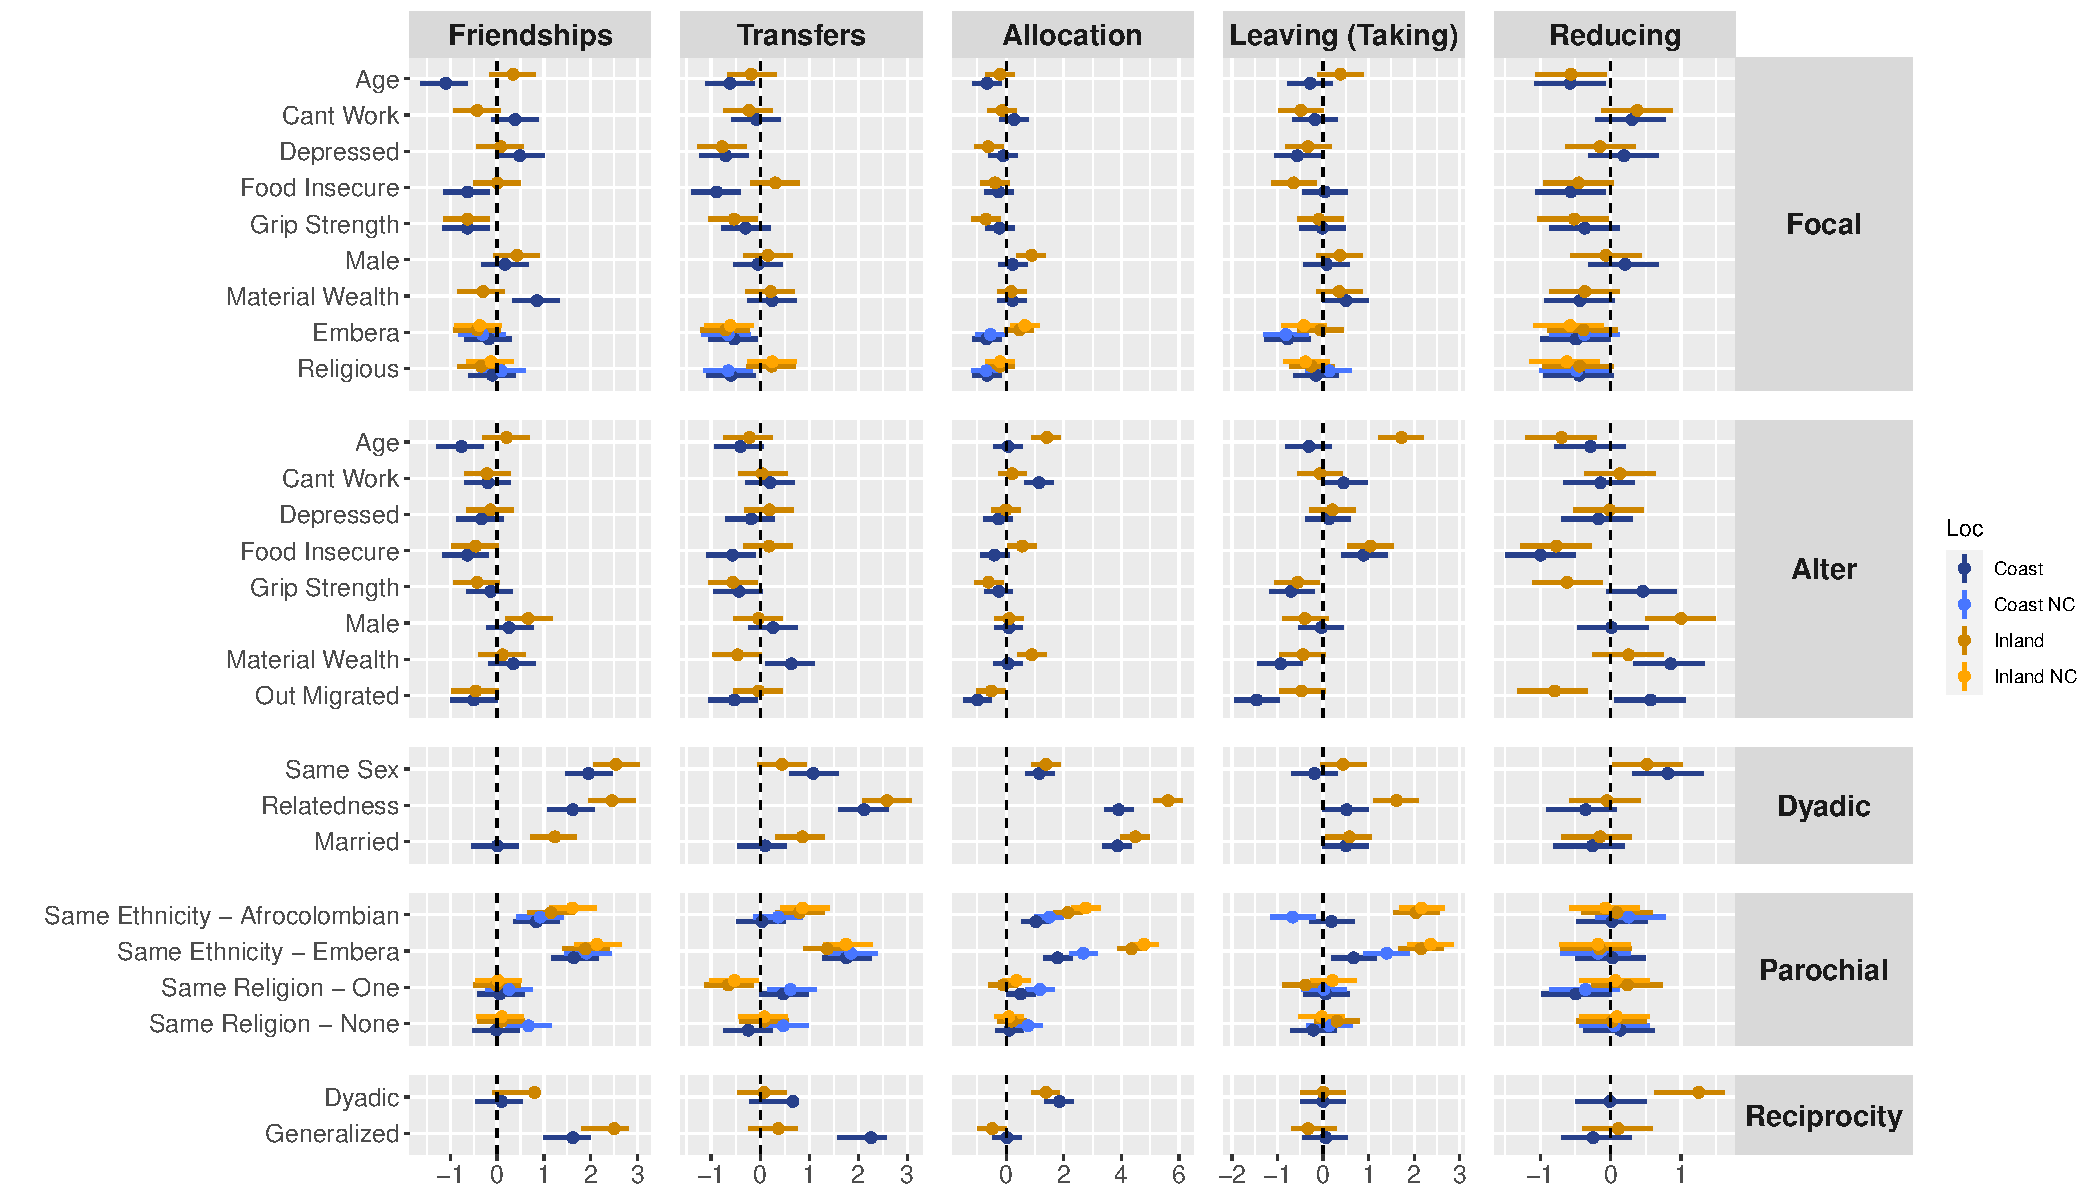
\includegraphics[width=6.5 in]{All_Games-Standardized_SRM} % this command will be ignored
\caption{{\footnotesize Multinomial regression results (standardized coefficients) from the Social Relations Model. Points and line-ranges show the standardized effects of predictor variables on outcomes (as medians and 90\% credible regions). Each column indicates an independently modeled outcome variable: i) friendship/socializing ties, ii) food/money transfers, iii) coin allocations in the allocation game, iv) coin deductions in the taking game (coded so that positive parameter estimates reflect \textit{leaving} coins), and v) coins paid to reduce an alter in the costly reduction game. For each of these outcomes in each community, CTR fit two models: both included the predictors directly related to parochial altruism (e.g., as in row 4), but the first (NC; \textit{No Controls}) excluded control variables (that is, the predictors in all other rows, except being religious and being Ember\'a (row 1)) and the second included controls. }
} \label{colombianres}
\end{figure*}

\ref{q1} \emph{To what extent does ethnic and religious parochialism structure social relationships, altruistic giving, exploitation, and costly reduction?} While ethnic identity and religiosity both structure social relationships and game play, the effect of ethnicity is more pronounced, especially in the inland community. From the perspective of Ember\'a individuals in both communities, ties---be they friendships, transfers of food or money, or transfers of coins in the RICH allocation and taking games---are more likely to be directed towards other Ember\'a than toward Afrocolombians. Afrocolombians at the inland community also preferentially form friendships with and give to other Afrocolombians; however, this effect only partially holds in the coastal community, where food and money transfers (column 2) as well as transfers in the taking/leaving game (column 4) show no evidence of parochial preferences.

 Religious individuals in the coastal community are more likely to make transfers of food and money to other religious individuals (column 2), are more likely to allocate coins to other religious individuals in the allocation game (column 3), and are less likely to punish other religious individuals in the costly reduction game (column 5). These effects, however, do not replicate in the inland community, where religious individuals were more likely to transfer food and money to \textit{non-religious} individuals. 
 
 In short, ethnic group membership clearly structures social relationships and game play at both sites, especially for the Ember\'a, while religiosity has less consistent and pronounced effects. Lastly, there is no clear ethnic pattern of costly reduction directed at either in-group or out-group members in either community.


\ref{q3} \emph{How do self-report data about food and money transfers compare to data collected with experimental economic games?} We first compare the effects described in the self-reported food and money transfers model (column 2) to those described in the allocation game model (column 3), as these measures correspond to making resource transfers in a context of economic constraint---in the real world, an inability to give food or money to everyone, and in the game context, too few coins to give to all alters. Many predictors, especially the dyadic ones (row 3), are consistent between  outcomes. The results also suggest similar patterns of parochialism (row 4), with the qualification that there is weaker evidence of parochialism in food/money transfers than in allocation game decisions among Afrocolombians in the coastal community. Turning our attention to parochialism in the leaving game (column 4), where deciders could leave coins for \textit{all} alters if they so chose, we again see comparability between predictors of self-reported transfers and predictors of coins left for recipients, supporting the external validity of the RICH games.

\ref{q2} \emph{How responsive is parochialism to varying cultural contexts---especially those owing to the relative wealth and population size of interacting groups?} When comparing the parochial altruism apparent at the coastal and inland communities (row 4), the effects in the leaving (column 4) and self-reported food/money transfer models (column 2) stand out. In the leaving game, where coins \textit{taken} benefit the decider at the expense of an alter, both Afrocolombians and Ember\'a at the inland community are more likely to take coins from out-group members than in-group-members; however, on the coast, model estimates suggest that Afrocolombians are either just as likely to leave coins for Ember\'a  as for Afrocolombians (model with controls) or are \textit{more} likely to leave coins for Ember\'a than for Afrocolombians (model without controls).  Afrocolombians in the inland community show parochialism in food/money transfers---a fact that may reflect a common \citep[although not universal,][]{Cay73} rejection of inter-ethnic demand sharing requests---while Afrocolombians in the coastal community show no such parochial preference and commonly engage in inter-ethnic giving.  We discuss further qualitative evidence concerning these key findings and provide more details about the relevant differences in cultural context in section \ref{qual}. 

\ref{q4} \emph{Are preferences for in-group cooperation decoupled from preferences for out-group exploitation and cost imposition?} Social-network data on existing relationships (e.g., friendship ties (column 1)) or giving (e.g., food/money transfers (column 2) and allocation game play (column 3)) can provide insight into in-group favoritism. To gain insight into \emph{negative} ties, it is useful to study other kinds of behavior, like exploitation (e.g., the taking game (column 4)) or direct cost imposition (e.g., the costly reduction game (column 5)). Data on food/money transfers, allocation game play, and friendship ties generally suggest in-group favoritism with respect to ethnic group members, although not (necessarily) with respect to alters who are similarly religious. In other words, same-ethnic-group favoritism in time and resource allocation appears quite robust in this data set. Additionally, as discussed above, Ember\'a at both sites and inland Afrocolombians are also more willing to generate costs for out-group than in-group members in the taking game, consistent with the predictions of models of parochial altruism.  However, we see no evidence of elevated out-group exploitation among coastal Afrocolombians. We also see no evidence of out-group bias in costly reduction in either ethnic group, in either community. As such, parochialism in out-group exploitation and especially out-group cost imposition seems to  be decoupled from in-group cooperation in these communities.

\ref{q5} \emph{To what extent can apparent parochial altruism be explained by individual and dyadic covariates?}
We find that estimates of parochialism (row 4) are surprisingly robust to the inclusion of controls for material wealth, food security, marriage ties, and genetic relatedness that could otherwise generate ``epiphenomenal'' parochialism, especially in contexts like the RICH allocation game, where the resources that can be distributed are much fewer than the set of possible recipients. In one case to the contrary, however, the apparent  ``anti-parochialism'' in leaving coins---i.e., the preferential leaving for Ember\'a alters by Afrocolombians in the coastal community---is attenuated when accounting for control variables. As these control variables include the material wealth and food insecurity of the alter, the reduction in the effect size of ``anti-parochialism'' upon inclusion of controls might indicate a mediating role of economic need at the coastal site in driving transfers from Afrocolombians toward Ember\'a.



\subsubsection{Qualitative accounts}\label{qual}
In post-game interviews in both communities, the most common explanation for game play behavior was the heuristic \textit{take from those who are better off and can afford it, and leave for those who are worse off and  need the money more. } In this light, the across-the-board parochialism of Ember\'a participants in both communities is explainable by the fact that, compared to local Afrocolombians, the Ember\'a live on more marginal lands, under more precarious economic circumstances, and in smaller, closer-knit groups where need and well-being are known. As we will see in section \ref{boliviagame}, just like the Tsimane' in Bolivia, Ember\'a give to, and leave for, those they see as most in need: other Ember\'a.

When asked in post-game interviews to explain their rationales for taking from whom they did, it was common for coastal Ember\'a respondents to emphasize taking from ``those who already have money to live on'' or ``those who have jobs,'' and leaving for ``people  in similar or worse situations to [themselves]'' and ``[their] neighbors who are also poor.'' Some coastal Afrocolombians also specifically mentioned out-group ethnicity as a motivation for \textit{not} taking coins: ``[I left coins for] the indigenous, the sick, and people of old age'', grouping Ember\'a residents into the class of people deserving of special consideration. Afrocolombians and Ember\'a at the coastal site both agree on whose relative need is greater; accordingly, Afrocolombians did not show evidence of parochialism in real-world food/money transfers or in experimental exploitation decisions in the RICH taking game. Qualitative responses in the coastal community focused on objective need and carried little emotional valence.


Similarly, in the inland community, Ember\'a participants agreed that Ember\'a alters were more in need than Afrocolombians and biased giving towards other Ember\'a accordingly. In stark contrast to the coastal community, however, it was very common in post-game interviews for Ember\'a respondents to describe taking from alters (normally Afrocolombians) specifically because those alters had not cooperated in the past, and there was clearly more social friction and negative emotional valence than in the coastal community. Ember\'a respondents would state that they took coins ``because these  are bad people  who don't cooperate'', ``because those people don't cooperate with you when you ask for help,'' or ``because they are bad people. You are hungry and ask for a favor and they do nothing.'' Though not recorded as explicitly in Afrocolombian's post-game interviews,  Afrocolombians in the inland community often imputed that Ember\'a alters from their community were as well off as the Ember\'a living in the nearby resguardo, causing them to engage in fewer inter-ethnic need-based or demand transfers, as is clear in both the experimental leaving game and real-world food/money transfer data.

%Although some of the content of the post-game interviews was similar at both coastal and inland sites---e.g., Ember\'a respondents would frequently describe taking from Afrocolombians who are comparably better off---the general tone was very different. This difference seems to arise from Ember\'a and Afrocolombian respondents at the coastal site having a shared perception of the correlation between need and ethnic group, while Ember\'a and Afrocolombian respondents at the inland site have different perceptions of who is most in need---and thus whether there is any obligation for Afrocolombians to provide food or money if requested by Ember\'a (or, similarly, whether there is any obligation to refrain from exploitation in the experimental taking game).  CODY: seems redudnant with above so I cut.

The findings presented here, both quantitative and qualitative, contrast in some ways with the \textit{simbiosis cultural} reported by \citet{Cay73}. By integrating community-wide self report and experimental data, along with qualitative debriefing interviews and standard ethnography, we have been able to build a more representative understanding of inter-group relationships. At a large-scale, the characterization of inter-group relationships as a \textit{simbiosis cultural} remains valid, as direct hostilities between groups are quite rare, and in both locations inter-group cooperation occurs between specific individuals on an almost daily basis. However, focusing only on a handful of easily observable cooperative relationships would obscure the larger picture, that on average, relationships in the inland site are rather parochial.
  

\subsection{Discussion}
\subsubsection{Mixed evidence for parochial altruism}

Consistent with our review of the parochial altruism literature (section \ref{onepointone}), our findings here demonstrate mixed evidence for ethnic and religious parochialism---across communities, groups, and data elicitation methods.

Friendship ties suggest a high degree of social assortment on the basis of group identity; this parallels similar findings at other sites \cite[e.g.,][]{power2017social, baerveldt2007ethnic}. Despite Afrocolombians and Ember\'a living in close proximity to each other in both communities, socializing is primarily confined to within-ethnicity interactions. These data correspond to historic accounts of a paucity of inter-ethnic marriages despite a long history of social contact \citep{Cay73}, and genetic evidence that shows a high degree of population substructure in the Pacific region of Colombia, in contrast to the Caribbean region where genetic admixture is high \citep{ossa2016outlining}.

Consistent with the social network data, when a small windfall of money was provided to respondents in the RICH games, this money was allocated primarily to same-ethnicity alters---an effect that was robust to controls for other measures of social proximity, including marriage and kinship. Based on such findings, one might conclude that individuals have a general predisposition to direct time and aid to coethnics.  However, the observed cross-site variation in parochialism in food/money transfers and exploitation ties highlights the flexible nature of the in-group/out-group distinction and illustrates how our choice of method might influence the weight of evidence for parochial altruism. Moreover, data on costly reduction suggest an absence of direct inter-group animus in both sites. In sum, the data suggest that expression of parochialism is context dependent, sensitive to the method of measurement, and that positive ties to same-ethnicity alters can be decoupled from negative ties to other-ethnicity alters.

\subsubsection{Relative population size, resource competition, and the cultural context of interactions}
\label{contextcc}
The coastal community is characterized by Afrocolombians having higher population size, more stable land tenure,  stronger local political institutions, and greater control of the means of production (i.e., fishing boats, refrigeration). In contrast, the inland community, on the ethnic boundary, is characterized by Afrocolombians and Ember\'a both having substantial population sizes, stable land tenure, and more comparable bargaining power. 

Although between-group resource competition is thought to be an important driver of parochialism  \citep{bellmoya} and there is greater scope for such competition at the inland site where population size and institutional power are more balanced, this explanation is not particularly relevant for these two sites because between-group resource competition is not a central feature of the cultural context. This being said, resource competition \textit{has} been cited for the breakdown of inter-ethnic cooperation between these same two ethnic groups in other regions of Colombia \citep[e.g.,][]{ng2000titling, davis2002indigenous, garcia2009diversos, velasco2011contested}. As such, it is likely that when there is more intense inter-group competition---i.e.,  direct legal conflict over land or resources---there will be a greater number of positive in-group ties and negative out-group ties \citet{choi2007coevolution}.

Likewise, the contrasting inter-group relationships at the coastal and inland sites is concordant with the predictions of some models of inter-ethnic coordination games \citep[e.g.,][]{mcelreath2003shared, advani2015melting}; these models suggest that when two ethnic groups are large enough, within-group interactions will occur more frequently than between-group interactions, such that the groups remain distinct sub-populations with their own behavioral norms \citep{bunce2017interethnic, bunce2018sustainability}. Ethnic groups are also predicted to remain distinct at their boundaries if benefits to in-group interaction are high \citep{mcelreath2003shared}. % Cody: I changed the preceding sentence because it was written as if McE et al predicted something about comparable group size, but I didn't see anything about that in my (admittedly brief) revisiting of that paper. But I might be wrong! Feel free to revert if so :).
Again, however, there is no ethnographic indication that coastal vs inland variation in parochialism is driven by such dynamics. Instead, the role of relative population size on expression of parochial preferences seems to be linked to the widely shared understanding that transfers should be based on relative need.




\subsubsection{Need-based transfers and inter-group relations}\label{discneed}

In both communities, formal statistical analysis and qualitative post-experiment interviews identified a key norm governing transfers---\textit{take from those who are better off and can afford it, and leave for those who are worse off and need the money more}---a classic, need-based heuristic found across a variety of cultural groups
\citep[e.g., ][]{peterson1993demand, hooper2015inclusive, aktipis2016cooperation, hao2015need, gervais2017rich, cronk2019managing}. This need-based norm appears more salient to respondents than a group-identity-based norm.

Inter-ethnic, need-based transfers, like those described at the coastal site, may be explainable by models of tolerated theft [though cf.]\citep{hao2015need}. Imbalance in marginal fitness benefit of a small food/money transfer has the potential to lead to conflict, as a resource-poor individual may be willing to escalate their demands for an essential resource from a resource-rich individual; this dynamic can lead to need-based transfers, whereby a well-off giver from a well-off group shares a resource whose benefit to an impoverished receiver from an impoverished group exceeds the cost to the giver of defending that resource \citep{jones1984selfish, winterhalder1996marginal, winterhalder1997gifts}.

 If ethnicity and need are perceived to covary, then members of a relatively well-off group may use ethnicity as a marker to direct need-based transfers, attenuating the overt expression of parochialism. In the coastal community, Ember\'a are a small proportion of the population and there is large between-group, but little within-group variation in wealth; ethnicity thus covaries strongly with perceived need. Coastal Afrocolombians and Ember\'a both recognize that the social obligation to help the needy means that resources should flow towards Ember\'a.  In the inland community, however, district-level population sizes are more balanced, and within-group variation in wealth and influence (e.g., comparing in-sample Ember\'a to those living on the resguardo) is higher. Here, ethnicity does not covary with perceived need and thus fails serve as an indicator that can be used to guide transfers. As such, inland Afrocolombians and Ember\'a are both more likely to cite need when directing resources towards members of their own group. 

\subsubsection{Religious parochialism}\label{relig}

Parochialism on the basis of religious group membership also appears to be flexible and responsive to cues of inter-group conflict, e.g., over land or resources. For example, reviewing the literature, \citet{lang2019moralizing} conclude that ``some studies showed that participants affiliated with religions emphasizing universal morality embrace the extension of cooperation behavior to out-group members \citep{preston2013different, ginges2016thinking, clingingsmith2009estimating, mccullough2016christian}, while other studies indicated that religious participants reveal hostility toward religious out-groups \citep{bushman2007god, shaver2018boundaries}'' [p. 2]. 

In the coastal community, both food/money transfers and game allocations were more likely to be directed, and costly reductions less likely to be directed, to other religious individuals. These effects did not replicate in the inland community, where food/money transfers were actually more likely to flow from religious individuals to non-religious individuals. It is possible that deeper within the Afrocolombian territory (where the coastal community is located), a focus on within-group solidarity coupled with a cultural context of resistance to hostile actors [see section \ref{pops}] \citep{oyola2017local} served a key role in fortifying relationships among the religious in-group. However, (i) sample size was insufficient to assess whether in-group favoritism was specifically directed toward members of the same church (e.g., the Catholic church), and (ii) more detailed ethnographic investigation of the churches of interest, along with targeted post-experimental interviews with religious respondents, would be needed to validate such explanations.


\section{Inter-group versus long-distance relationships in lowland Bolivia}
\subsection{Assuming parochial altruism}
ACP began studying inter-group relationships in Bolivia in 2010, with a focus on when and why   individuals form cooperative relationships with people outside of their communities.   She focused on Bolivia for two reasons. First, after three decades of large-scale movements pushing for Indigenous rights, the federal government of Bolivia came to recognize the sovereignty of 36 different  \textit{pueblos ind\'igenas}---Indigenous groups whose members are \textit{originarios}, living on their traditional lands, and whose members share cultural institutions (explicitly recognized by the government as their  \textit{usos y costumbres}), making ``\textit{pueblo ind\'igena}'' akin to the definition of ``ethnicity'' used in the parochial altruism literature. However, because the state preferentially allocates its limited funds to \textit{originarios}, new lines of competition have been drawn \textit{between} some Indigenous groups. What was a superordinate identity of indigeneity in the 1980s--2000s has splintered as \textit{pueblos ind\'igenas} now compete with one another for resources and recognition \citep{fontana2014indigenous}.
Second, Evangelical churches of various denominations are expanding their presence in Bolivia \citep{lesley1993religious}, as elsewhere in Latin America \citep{stoll1990latin}; rural Bolivians candidly contrast Catholic and Protestant beliefs, distinguishing what ``we'' do from what ``they'' do that ``we'' would never do. 

In the midst of these changes, market participation is on the rise among slash-and-burn horticulturalists living in the lowlands as these populations rely less on subsistence production and more on cash income or trade to acquire food and other goods \citep{gurven2015does, reyes2010integration}. With increased market participation comes increased mobility, contact with middlemen, and exposure to individuals in other \textit{pueblos ind\'igenas} and who live far away \citep{pisorjones2020}.

 Adopting the assumption from the parochial altruism literature that ethnic groups are containers for cooperation (section \ref{onepointone}), ACP set out to study when and why cooperative relationships might transcend the boundaries of \textit{pueblos ind\'igenas} or, given its increased relevance, the Catholic/Evangelical divide. She hypothesized that individuals with fewer resources might be more likely to exhibit preferences for building relationships with out-group members---in other words, that their interest in potential resource access might act as an ``override'' to parochialism [see section \ref{onepointone}] \citep{pisor2016risk, pisor2018diversify}. This hypothesis was partially supported. However, it was short-sighted.

\subsection{Collaborating communities in Bolivia}\label{pops2}
Three populations of horticulturalists---the Moset\'en, the Tsimane’, and the Interculturales---are the focus of the present study. The Moset\'en and Tsimane’ are \textit{pueblos ind\'igenas}, recognized by the Bolivian government as \textit{originarios} because they live on their traditional lands. The Moset\'en and Tsimane’ have lived in the lowlands for centuries  \citep{godoy2015natural, tomas2008tsimane}, and the two groups were once a continuous, intermarrying population \citep{bert2001major, godoy2015natural, gurven2007mortality, sakel2011moseten, ringhofer2010exploring}. 

Today, however, their lives are quite different. While the Moset\'en were missionized by Franciscan Catholics during the 19th century \citep{godoy2015natural, mamani2010tsinsi, ref947717999}, the Tsimane' were missionized in the 20th century by Evangelical Christians \citep{tomas2008tsimane}. Efforts by missionaries resulted in access to roads and secondary education for most Moset\'en communities by the year 2000 \citep{pisor2018diversify}; in contrast,  only a minority of Tsimane' communities have access to major roads or secondary schooling \citep{ringhofer2010exploring}. 
The Moset\'en have more years of education, participate more in the market economy, and have higher mobility than do the Tsimane'. Today, while the Moset\'en speak fluent Spanish, the \textit{lingua franca} among the different \textit{pueblos ind\'igenas} of Bolivia, and intermarry extensively with other \textit{pueblos ind\'igenas} \citep{pisor2018diversify}, only 14\% of the Tsimane' speak fluent Spanish \citep{pisor2016risk} and few have intermarried with other \textit{pueblos ind\'igenas}.

The Interculturales are another community of horticulturalists of Indigenous descent. The word \textit{intercultural} is a designation used by the Bolivian government to recognize communities who are no longer on their traditional lands \citep{albo2007bolivia}; they are not considered \textit{originarios} and are not eligible for special government recognition and resources. The Intercultural community discussed here is composed primarily of descendants of the Aymara and Quechua \textit{pueblos ind\'igenas}. These groups moved to the area during government relocation programs in the 1950s--60s or during booms in the logging and quinine industries  \citep{pisor2016risk, pisor2018diversify}. Upon arrival, many Interculturales learned horticulture for the first time, sometimes by copying the Moset\'en. However, they retained many Aymara-influenced institutions, especially with respect to social and political organization. The Interculturales are more reliant on the market economy than are the Moset\'en: they have had reliable access to roads for 25 years longer \citep{Llojlla2011} and they began to build economic relationships with middlemen much earlier \citep{pisorjones2020}. On average, the Interculturales have as much education as the Moset\'en but slightly higher incomes, more market possessions, and higher mobility.
		  

\subsection{A game with many interpretations}\label{boliviagame}

In 2014 and 2015, ACP and Michael Gurven used a non-anonymous economic game to assess whether members of the Moset\'en, Tsimane', and Interculturales were less likely to favor in-group members---individuals of the same \textit{pueblo ind\'igena} or religious affiliation---if they stood to gain more from out-group members, whether in access to income or  market goods \citep{pisor2016risk, pisor2018diversify}. %ACP interviewed participants from two Moset\'en communities, three Tsimane' communities, and one community of Interculturales.
 Participants were presented with photos of six strangers, three from their in-group and three from their out-group, and told the first name, age, and either \textit{pueblo ind\'igena} or religious affiliation of each. ACP then placed three coins (each worth \$0.14 USD; total stakes: 1/3 of a day's wages) on each photo, and three coins in front of the participant; she told them that they could move any coins they wished, and that any coins left on a photo would be given to that person in the participant's name. Any coins the participant left in front of themselves would be theirs to keep. The intention of this method was to assess participants' preferences for forming a new relationship with an in-group stranger versus an out-group stranger through an act of generosity, in a task that explicitly pitted in-group favoritism against the possibility of out-group relationships. For further details on this method, see \citet{pisor2016risk, pisor2018diversify}.

ACP and Gurven found that participants who felt that they were subjectively less well-off relative to others in their community were more likely to give money to out-group members \citep{pisor2016risk}. Though participants gave more to in-group members than to out-group members on average, mean out-group giving was far from zero: 82\% of participants gave at least some money to out-group members \citep{pisor2018diversify}. %\footnote{This may have been due to priming concepts of fairness, as the initial allocation was three coins per person. That said, participants were unlikely to award 3 coins to each recipient; instead, most moved at least one coin, perhaps because they felt they had to do something \citep{list2007interpretation}. Tsimane' participants also behaved quite differently from the Moset\'en and Interculturales.}. 
Per our discussion of the role of religious institutions (section \ref{relig}), frequency of church attendance predicted giving more to out-group members, but only for the Interculturales \citep{pisor2016risk}. However, these patterns of out-group giving had caveats. First, Tsimane' preferences looked quite different from Moset\'en and Intercultural preferences. Tsimane' participants were far less likely to give any money to individuals of other \textit{pueblos ind\'igenas} or  religious affiliations\footnote{Note that at the time of data collection, most Tsimane' affiliated themselves with the same Evangelical church, such that recipients of the same religious affiliation were frequently also Tsimane', something the participants could detect from looking at the photos \citep{pisor2018diversify}.}. Perhaps this behavior was a product of the use of money in the experimental task; the Tsimane' have less wealth than the other groups and see themselves as the ``have-nots''  \citep{pisor2018diversify}. However, while participants from all three populations who felt they had fewer resources than others gave more to out-group strangers, only the Tsimane' gave more to out-group strangers if they also had fewer market items  (Figure \ref{boliviamarket}). Finally, group membership was not the only basis for decision-making. In post-decision interviews, participants---especially Moset\'en and Interculturales---described inferring recipient characteristics from their photos, including their relative need and whether they were a good person, in order to make decisions \citep{pisor2018diversify, Pisor2020}.

 \begin{figure}[t]
	\centering
	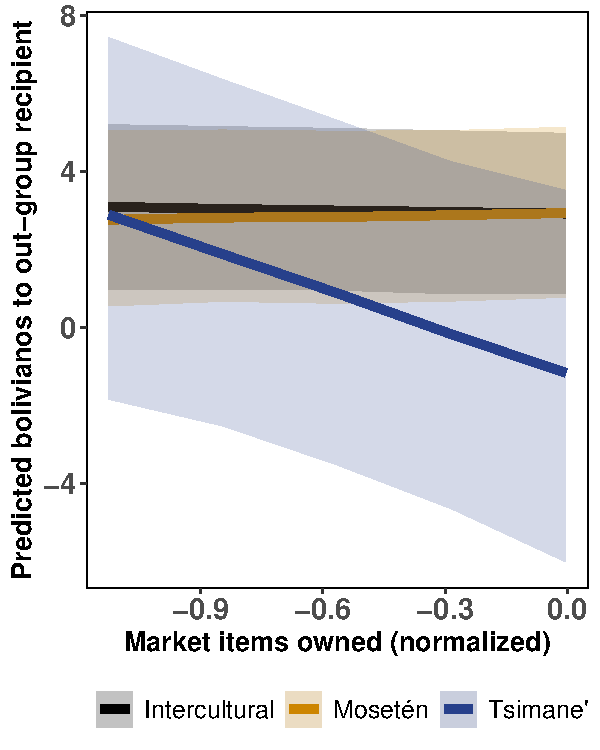
\includegraphics[width=2.1in]{Market_items}
	\caption{{\footnotesize Predicted \textit{bolivianos}, the local currency in Bolivia, given by a participant to an out-group stranger (that is, an individual from another \textit{pueblo ind\'igena} or with a different religious affiliation) as a function of the total estimated value of market items owned by the participant, normalized relative to other participants in the same population \citep{pisor2016risk, pisor2018diversify}.}} \label{boliviamarket}
\end{figure}

This contrast in generosity toward out-group members was foreshadowed by our overview of these three populations in section \ref{pops2}: the Tsimane' have fewer interactions with members of other \textit{pueblos ind\'igenas} than do the Moset\'en or Interculturales. Some of this is due to their constrained mobility, given their limited access to roads and to income to purchase gasoline for river travel. Some of this is due to their lack of access to education, keeping the percentage of fluent Spanish speakers low. But some of this is also due to choice. At the time of European contact, the Tsimane' were well-known among other Indigenous groups in the region as salt traders \citep{godoy2015natural,  ref947717999}. However, their interactions with highland Bolivians (\textit{collas}) and non-Indigenous lowland Bolivians (\textit{cambas}) have been marked by misunderstandings, marginalization, and discrimination; the Tsimane' physically retreated from contact with the Spanish and \textit{cambas} multiple times when these groups took advantage of them \citep{godoy2015natural, ringhofer2010exploring, tomas2008tsimane}. 

Though Tsimane' participants with fewer market possessions gave more to out-group members, supporting ACP's hypothesis about strategically building between-group relationships to gain resource access, it may be instead that Tsimane' participants who are more involved in the market economy have more exposure to discrimination at the hands of out-groups and are thus more parochially altruistic \citep{pisor2018diversify}. When asked about \textit{collas} and \textit{cambas}, many Tsimane' talked about their access to market resources and their encroachment on and destruction of Tsimane' land \citep{pisor2018diversify}. However, when asked about their game decisions, Tsimane' participants reported that their decision to give more to Tsimane' recipients than to recipients from other \textit{pueblos ind\'igenas} did not reflect a wish to benefit the Tsimane' at the expense of other groups, per the tenets of parochial altruism; rather, like the coastal Ember\'a in Colombia (section \ref{discneed}), the participants reasoned that those groups already had plenty of money, so they wished to give the Tsimane' more for themselves \citep{Pisor2020}.
	

\subsection{Conflating two questions}\label{twoquest}

Although market participation is increasing for all three populations, none of these populations are interacting with other \textit{pueblos ind\'igenas} for the first time. The Tsimane' were renowned traders before the 20th century. The Moset\'en have long traded with lowland groups for tools, medicine, and plants \citep{lathrap1973antiquity, ringhofer2010exploring} and, centuries ago, with the Inca for metal goods \citep{godoy2015natural}. Before  Columbus, the Quechua and Aymara (whose descendants are residents of the Intercultural community) had trade networks spanning the Andean ecozones, ensuring access to foods from different regions \citep{klein2011concise}. Note that key benefit of these relationships is not necessarily that they cross ethnic boundaries, but that they span distance: for example, highland Aymara residents would often trade with lowland Aymara ``colonists.'' ACP had conflated two orthogonal questions about sociality in her work: whether people respond to a lack of resource access with increased preferences for forming long-distance   relationships, and whether a lack of resource access diminishes parochial altruism.

Why is it important to distinguish study of the evolution of long-distance relationships from the study of between-group relationships in humans? Because both resource competition and resource sharing have been important selection pressures over the course of human evolution, and both have likely affected the psychological adaptations we have for evaluating friend and foe---including both our propensity toward parochialism \citep{hruschka2013economic} and our propensity for strategically building long-distance relationships when they are beneficial \citep{pisor2019evolution, pisorjones2020}. Having long-distance relationships is a means to maintain consistent access to resources, something especially important in humans given our high energy throughput and need for specific nutrients and minerals \citep{pisor2019evolution}. By forming relationships outside their communities, individuals can access resources not locally available---like salt, which, in the Amazon was heavily concentrated in certain areas \citep{reeve1993regional}---or manage the risk of shortfalls that can strike entire communities, e.g., those created by floods or droughts \citep{pisor2019evolution, pisorjones2020}. How ``long'' is long-distance enough to provide non-local resource access and buffer shortfalls depends on the ecology (e.g., how diverse resources are locally), whether different individuals specialize in the production of different resources, and the spatial scale of shortfalls \citep{pisorjones2020}. Ethnic boundaries, the group divisions most commonly investigated in the parochial altruism literature (section \ref{onepointone}), can be pronounced both in the contexts of between-group resource competition \citep{choi2007coevolution, bellmoya} \textit{and} between-group sharing, when the efficiency of production may be increased if different ethnic groups focus on different products, favoring specialization and resource exchange \citep{barth1956ecologic, brewer1976ethnocentrism, bowles2004persistent}. Long-distance relationships often span ethnic boundaries; even where ethnic divisions are marked, if long-distance relationships benefit individuals, cultural institutions may permit inter-group social connections \citep{bollig2010risk}, or intrepid individuals may forge their own \citep{pisor2019evolution, schaub2017threat}.


Distinguishing between these two research foci---the evolution of long-distance relationships and the evolution of between-group relationships---helps to clarify three of most common reasons given for why parochial altruism varies across individuals and groups (section \ref{onepointone}). When the benefits of long-distance social relationships or inter-group specialization exceed the costs, parochial altruism can be overridden \citep[e.g.,][]{bellmoya}. This can result from individual preferences to interact with distant individuals \citep{pisor2019evolution} or out-group members \citep{moya2015different, brewer1976ethnocentrism} or, as noted in section \ref{onepointone}, by cultural institutions enforcing inter-group tolerance \citep{fearon1996explaining, fry2018evolutionary}. Though differences in norms between ethnic groups may increase the costs of coordination between them \citep{bellmoya, habyarimana2007does, mcelreath2003shared}, if between-group relationships are beneficial enough, the norms that increase these costs may be lost \citep{bunce2017interethnic, bunce2018sustainability}. These models help clarify diffuse arguments about why individuals develop additional loyalties when exposed to people from other ethnic groups or other countries \citep[e.g.,][]{brewer1976ethnocentrism, beck2006cosmopolitan, hruschka2013economic, buchan2009globalization, fukuyama2001social, mau2008cosmopolitan, singer2011expanding}.

Note that the strategic building of long-distance or between-group relationships to gain access to resources not locally available is distinct from the material security hypothesis \citep{hruschka2013economic, hruschka2014impartial}. This hypothesis suggests that individuals who do not have their basic needs met---including maintaining health and having enough food and money---will be more in-group favoring by not following impartial rules \citep{hruschka2014impartial}. Between-group or long-distance relationships are often not an efficient way to meet basic needs \citep{minnis1985social}; instead, individuals may preferentially invest in in-group relationships because, in the absence of state support, basic needs can be met through localized cultural institutions for managing risk \citep{pisorjones2020}. Long-distance relationships are often forged and maintained when the benefits gained through them (usually in terms of non-local resource access) exceed maintenance costs \citep{pisor2019evolution}; the same is true of the gains-to-trade made possible by inter-group relationships \citep{bellmoya}.

As ACP realized her interest in how individuals improve their non-local resource access was really one of forging \textit{long-distance relationships}, not necessarily \textit{between-group relationships}, she returned to Bolivia in 2017 to investigate this clarified research question. Given how different the Tsimane’ were from the Mosetén and Interculturales in their mobility and market participation---not to mention their game play in 2014---ACP focused on the Interculturales and the Moset\'en in 2017.
	
	\subsection{The reality of long-distance relationships}\label{distance}
	Though long-distance relationships can be important both for maintaining access to non-local resources and for buffering local shortfalls \citep{pisor2019evolution}, long-distance relationships have not proven relevant for buffering local shortfalls among the Moset\'en and Interculturales \citep{pisorjones2020}. In 2014, both the Moset\'en and Intercultural communities (and much of lowland Bolivia) were hit with severe flooding and landslides, severing roads and cutting power and cell service for more than a month. Although floods usually occur with less intensity, both the Moset\'en and Interculturales have cultural practices for managing the risk of resource shortfall due to flooding, including raising pigs and chickens that can be slaughtered during hard times and, for the Interculturales, a system of loaning bags of rice to neighbors with expected deferred reciprocity of bags returned the next year. When fallback foods were mostly depleted by the flood in 2014, rather than calling on long-distance relationships---which could not be reached, due to lost roads and lack of cell service---the Moset\'en marched down their destroyed road to demand the support of the local government. Both communities eventually used motorized canoes to ferry emergency supplies from the local town. Once the waters receded and roads were repaired, community members who could not absorb the cost of their destroyed crops sought loans from local banks. Three years later, when asked who would help them with a loan during a future hypothetical flood, Moset\'en and Intercultural participants were more likely to name same-community individuals (or even the government) than connections at a distance (Figure \ref{boliviaflood}) \citep{pisorjones2020}. In short, because both communities maintain local institutions for managing risk and because both found no use for long-distance relationships during the last major flood, long-distance relationships do not appear to buffer shortfalls for the Moset\'en and Interculturales \citep{pisorjones2020}.

\begin{figure}[t]
	\begin{subfigure}{0.5\columnwidth}
		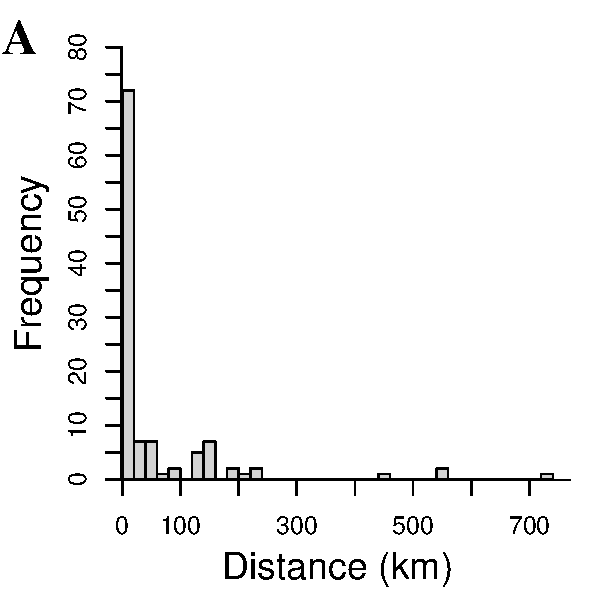
\includegraphics[width=\linewidth]{FloodHistogram.pdf}
	\end{subfigure}%
	\begin{subfigure}{0.5\columnwidth}
		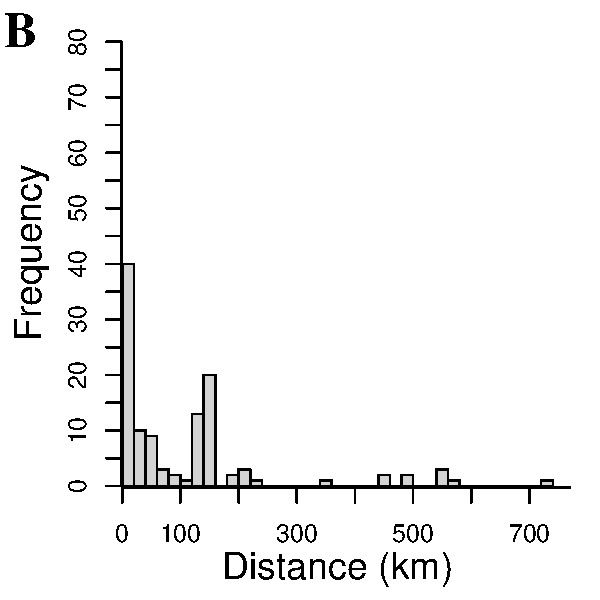
\includegraphics[width=\linewidth]{WorkHistogram.pdf}
	\end{subfigure}
	\caption{{\footnotesize Each participant was asked to name someone who could help them (a) with a loan of 500 \textit{bolivianos} ($\sim$\$70, or 8 days' wages) if a flood destroyed their crops, and (b) find ``a good job that pays well''; these counts reflect how far away these named individuals lived in kms.}} \label{boliviaflood}
\end{figure}

That said, for both the Moset\'en and Interculturales, long-distance social relationships are crucial for access to resources not locally available \citep{pisorjones2020}.
 First, both rely on middlemen, often based in the capital city of La Paz (seven hours away by car), to purchase their crops. Second, both increasingly participate in migrant labor to supplement their incomes. Extra-community connections are key to finding migrant labor work; when asked who they would contact for a ``good job that pays well,'' 65\% of participants named someone outside their community (Figure \ref{boliviaflood}). Third, market participation increases cash income, which translates into increased mobility. Urban social connections increase the financial and logistic feasibility of mobility. The Moset\'en and Interculturales increasingly have business in La Paz and increasingly send their children to university or job training programs. Individuals report that La Paz residents help them navigate local bureaucracy, from completing government paperwork to enrolling in university. Further, given the high cost of lodging in La Paz, urban connections can provide low-cost shelter. Fourth, urban connections provide access to goods only available in the city; e.g., La Paz residents frequently send parcels (\textit{encomiendas})---which can contain anything from bread to cell phones or televisions---by bus to rural residents.

	The Moset\'en and Interculturales maintain these long-distance relationships through a variety of means \citep{pisorjones2020}. Reciprocal exchanges of \emph{encomiendas} are common: residents of La Paz often request fresh produce like plantains and mandarin oranges, which are expensive in the city. Individuals also send or receive money transfers (\textit{giros}); \textit{giros} may be used to reimburse someone for an expensive encomienda or to loan money. Semi-reliable cell phone service has been available to the Moset\'en and Interculturales since 2010. Phone calls, and increasingly, WhatsApp or Facebook Messenger, are used to maintain contact with far-flung friends. Visitation remains important to relationship maintenance: depending on an individual's means, they may take buses, shared taxis, or their own vehicle to visit long-distance connections, often for several days.
	
	Who are these long-distance connections? Unsurprisingly, many are consanguineal kin (related by blood) or affinal kin (in-laws) \citep{pisorjones2020}. %Reciprocal relationships with consanguineal kin can be less difficult to manage (and thus less costly) than reciprocal relationships with unrelated individuals because of convergent fitness interests \citep{hruschka2010}. Important to note, however, is that an individual may selectively invest in relationships with certain consanguineal kin who can generate more benefits for them---for example, with particular siblings that are well-positioned to provide non-local resource access. Siblings were commonly named by Moset\'en and Intercultural participants as non-local connections who could provide information on a good job. Marriage can be strategically used to gain non-local resource access through one's spouse or affines \citep{pisor2019evolution, chapais2009primeval}. Some Moset\'en participants, for example, accuse non-Moset\'en men of marrying Moset\'en women to gain access to Moset\'en tribal lands. 
	However, Moset\'en and Intercultural Catholics strategically use fictive kinship---namely, godparent relationships (\emph{compadrazgo}; see section \ref{histcon})---to solidify long-distance connections with individuals they believe are wealthy or influential enough to help them or their children \citep{mintz1950analysis}; teachers, doctors, and middlemen, who are often from La Paz and spend time in both locations, are favorite choices. Long-distance friendships are also forged during periods of temporary migration: for example, during stints of migrant labor, while studying at university or in career programs, or, for men, while completing  military service.
	
	Interestingly, with respect to ``who'' these long-distance connections are, participants were often hard-pressed to identify the \textit{pueblo ind\'igena} of their friends. First, participants had a difficult time understanding the question: ACP often cycled through several phrases---\textit{pueblo ind\'igena}, \textit{descendencia} (descent), \textit{parentezco} (kinship)---before a given participant was able to answer. Second, participants often guessed at the response. Some identified all friends from the lowlands as \textit{cambas}, even though Indigenous peoples are also from the region; others reasoned that if someone lives in La Paz, they must be Aymara, the dominant \textit{pueblo ind\'igena} in the city. In short, the \textit{pueblo ind\'igena} of a long-distance social connection was far less salient to participants than might be expected given the political landscape in Bolivia. See \citet{moya2015different} for a similar example from Per\'u.

\subsection{A failed attempt at distinguishing distance preferences from group preferences}

Given the wealth of observational and self-report evidence that long-distance relationships are important to the Moset\'en and Interculturales, ACP set out to design a task that could potentially decouple participants' preferences for long-distance relationships from their preferences for between-group relationships. Drawing on marketing research, she chose a paired comparison choice-based task \citep{rao2014applied} to assess which traits participants preferred in candidate friends. Though individual-level differences in resource access may predict differential investment in long-distance relationships, and though participants' perceptions of group-level differences in wealth may affect parochial altruism (section \ref{twoquest}; see also the Colombian data, section \ref{qual}), ACP was also aware that participants with less wealth may have been more incentivized to keep money for themselves in the 2014--2015 economic game. She reasoned that a task not involving money might reveal preferences for forming new social relationships independently of preferences for giving or keeping money. She presented each participant with two cards representing two candidate friends, each with six different characteristics (see Figure \ref{boliviacards}); these included where the candidate friend lived, their \textit{pueblo ind\'igena}, and their religious affiliation. Participants made 18 sequential decisions between pairs of cards, from which we inferred their preferences for the characteristics of a new friend. See supplementary appendix section 3 for more details.


 \begin{figure*}[t]
 \centering
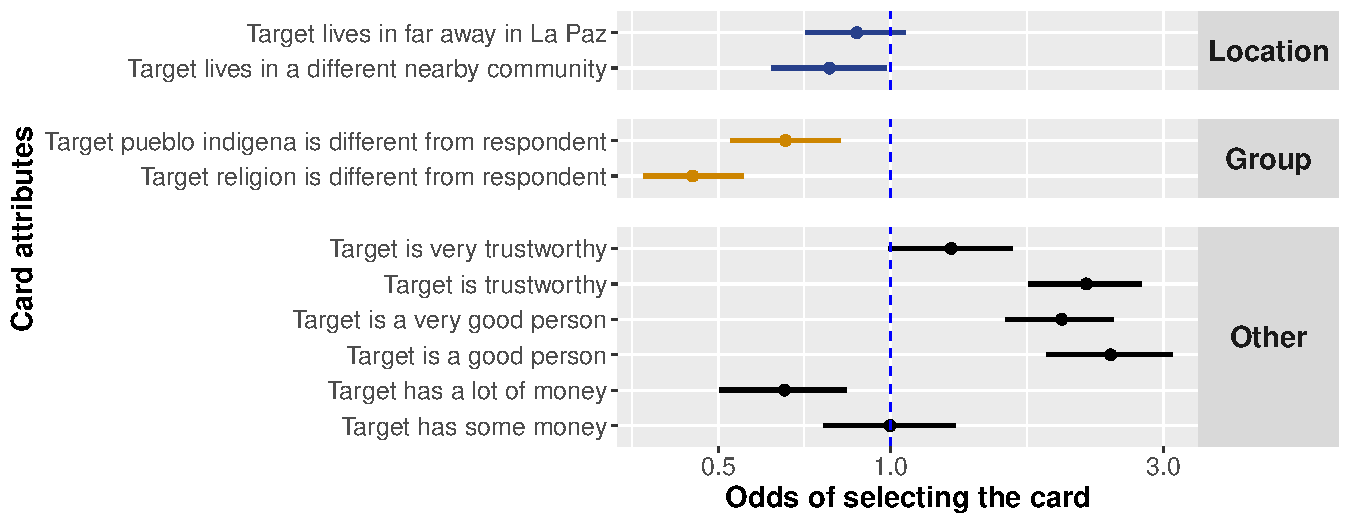
\includegraphics[width=5.2in]{Bolivia_CardChoice_Non-Standardized_CR} % this command will be ignored
\caption{{\footnotesize Each respondent was presented with two cards that each had several attributes, and was asked to indicate which card better described a desirable new friend. Some attributes were the same on both cards, others differed. Here, we present model estimates of the odds of selecting one card if it were to differ by only a single attribute from the other card. The base case is a candidate friend who lives in the same community, is from the same pueblo ind\'igena and same religious affiliation, and who is not good, not trustworthy, and has no money. The estimates indicate that participants preferred a same-community friend (the baseline) over more distant friends, same-ethnic and -religious group friends over those from other groups, and friends that are `good people', trustworthy, and---interestingly---not excessively wealthy. In sum, participants expressed parochial preferences in terms of both religion and ethnicity, and did not express preferences for long-distance friendships.
}
} \label{boliviacards}
\end{figure*}



	Participant preferences in the choice task did not reflect the documented prevalence of long-distance relationships in these communities (section \ref{distance}). A candidate friend's pueblo ind\'igena and religious affiliation were highly salient to participant preferences, with participants preferring candidate friends of their own pueblo ind\'igena and religious affiliation (Figure \ref{boliviacards}). Participants also had a slight, though inconsistent, preference for friends from their same community over friends from other places. 
	
	Why the discrepancy between the ethnographic reality and preferences elicited by the choice task? Some participants reasoned aloud during the decision-making process, providing some insight \citep{bernard2017research}. These participants would often identify one characteristic of the six that stood out to them (``this one is from my church, so I pick him'') and continue to make decisions based on that criterion across all pairs of cards. In other words, even though the characteristics of candidate friends varied across cards, participants stopped attending to characteristics other than the one they initially  selected. Not only did preferences in the choice task not reflect the documented preferences for long-distance relationships,  they did not reflect preferences elicited by the 2014--2015 economic game either. Recall that in the economic game, despite some in-group preference, there was substantial out-group giving. In total, 63 participants completed the 2017 choice task and the 2014--2015 economic game. Interestingly, there was no relationship between participants' preferences in the 2014--2015 game and their preferences in the 2017 choice task (see supplementary appendix section 3). Perhaps this difference in preferences was due to real changes in preferences over time, possibly related to political climate or changes in material wealth (see supplementary appendix section 3); however, it is likely at least partially due to the difference in methodological design.
	
	\subsection{Is parochialism in the method?}
How could these methods---observation, survey, an economic game, and a choice task---produce such discrepant results? While observational data reflect real-world behavior, as do self-report data (assuming participants respond accurately), neither the economic game nor the choice task were designed to capture behavior under real-world constraints; accordingly, we should not expect either to map onto real-world behavior  \citep{Pisor2020, gurven2008collective}. The economic game was designed to bring together strangers (the participants themselves and the recipients in the photos) in first-time interactions that might never occur in the real world, especially for Tsimane' participants, who speak little Spanish and participate less in the market economy. However, the game may have been more real-world than the choice task: the use of money in economic games incentivizes decision-making, such that participants feel their decisions have real-world outcomes \citep{guala2005methodology}. Further, for participants with little wealth who perhaps cannot afford to be generous in the real world, economic games provide an opportunity to give, eliciting participant preferences for giving that may usually be masked by real-world constraints (section \ref{qual}; \citep{Pisor2020}). ACP designed the choice task to remove all information about a candidate friend except the six characteristics described, which is not at all like how social partners are chosen in the real world \citep[see][for a relevant review]{barclay2013strategies}. Without monetary incentives to require that participants ``put their money where their mouth is,'' there was no cost to participants using any available  heuristic to navigate the choice task \citep{Pisor2020, xygalatasreligious}. For a related discussion about why methods that originate in Western academic contexts, like the choice task, may fail in the field, see \citet{hruschka2018learning}.

There are certainly reasons to use methodologies that do not approximate the real world, as we discuss in \citet{Pisor2020}; ACP hoped that by removing features of the real-world, such as the information in photos and the potential biases introduced by money, she could better understand participant preferences with minimal intrusion from real-world constraints. However, the choice task in particular deviated so far from the real-world constraints that might guide partner choice, ACP is not convinced that it provided much meaningful insight into participants' preferences for new social relationships.

	How do these results bear on the mixed evidence for parochial altruism that researchers have gathered from around the globe? As evidenced by our comparison of the Tsimane', Moset\'en, and Interculturales, parochial altruism does seem to vary, both across individuals and across ethnic groups. However, different methods used with the \emph{same} individuals suggest different degrees of in-group favoritism. For example, the way a task is explicitly framed---what researchers do (or do not) tell participants about the task---and its implicit features---whether the choice to give to an in-group member does or does not impact out-group members \citep{hagen2006game, lightner2017, Pisor2020}---have behavioral consequences. 
	Further, evidence from Bolivia and elsewhere suggests that social scientists may need to step away from the assumption that ethnic groups inevitably function as containers for cooperation \citep{moya2015different}. As we have argued here, distinguishing between different selection pressures that favor interest or disinterest in strangers---as ACP highlighted, separately investigating the roles of long-distance relationships and  between-group relationships---may help us parse the variability researchers have documented in studies of parochial altruism. If we wish to better understand human sociality, we need to take a step back, hone our hypotheses, and then purposefully design our data collection methods accordingly.



\section{General discussion}
%Introduced as a term two decades ago, parochial altruism---generating benefits for in-group members at out-group expense---has had wide-ranging influence on the study of human sociality in the social sciences. If the concept is so influential, however, why does parochial altruism seem to vary so much across individuals, communities, and studies? Institutions may offer one explanation as, when there are net benefits to cooperating with out-group members, this can favor the cultural evolution of norms and rules that further enhance the benefits of between-group interaction \citep{fearon1996explaining, fry2018evolutionary, pisor2019evolution}. Features of our psychology offer another possibility: perhaps because of the benefits they offer, we begin to see members of other ethnic groups as part of our in-group \citep{brewer1976ethnocentrism, beck2006cosmopolitan, buchan2009globalization, fukuyama2001social, hruschka2013economic, mau2008cosmopolitan, singer2011expanding}, or perhaps we can afford the time or resources to care about out-group members when our own needs have been met \citep{hruschka2014impartial, silva2014cooperation}. Yet another explanation stems from data suggesting that in-group cooperation does not always require out-group cost generation \citep{purzycki2019identity, hruschka2013economic, yamagishi2016parochial, brewer2006evolutionary, schaub2017threat, cashdan2001ethnocentrism, Rusch2014}---groups can compete by producing more benefits for their members than other groups do, without directly harming out-groups \citep{waring2015}. Importantly, however, the methods researchers use may be responsible for some of the observed variability in parochial altruism, making it difficult to disambiguate methodological from on-the-ground variation \citep{Pisor2020}.

We have drawn on two case studies from rural South America to explore variation in parochial altruism across communities, paying special attention to the effect of methodology.  We found differences in parochial behavior across ethnographic, social network, economic experiment, and choice task data. This is unsurprising, as some of these methods (e.g., ethnographic and social network data) measure real-world behavior, which is subject to numerous constraints, while others (e.g.,  economic games) better measure private preferences \citep{Pisor2020}. Parochial preferences varied across communities, across individuals, and even \emph{within} individuals across methods. Here, we review these results in light of the different explanations for on-the-ground variability in parochial altruism described in the introduction. We then turn to methods, exploring how minor differences in research design can impact research findings. Finally, we close by raising two relevant considerations for field researchers studying parochial altruism.

\subsection{Empirical variation in parochial altruism}

In the introduction, we identified three common explanations from the literature for the variation in parochial altruism. We return to these explanations here, reviewing their potential roles in explaining the data from Colombia and Bolivia, and exploring their relationship to another literature on cooperation: that of need-based transfers \citep[e.g.,][]{peterson1993demand, hooper2015inclusive, aktipis2016cooperation, hao2015need, cronk2019managing}.

\emph{Institutions:} In Colombia and Bolivia, some of the most relevant local institutions are churches. By fostering belief in omniscient deities that favor impartial rule-following, religions can instill norms of more equitable treatment towards individuals from other ethnic groups or of other religious affiliations \citep{purzycki2018evolution, lang2019moralizing}. That said, we saw little evidence that religiosity diminished parochialism in these communities. An exception was in the Intercultural community in Bolivia, where individuals who attended church more frequently were more likely to give money to individuals from other ethnic groups or religious affiliations. 

\emph{Basic needs:} Impartial treatment of out-group members is more likely to arise if individuals have their basic needs met; for example, if government programs buffer shortfalls due to environmental variability or lost jobs, individuals can better afford to share their resources with those of different, perhaps more marginalized groups  \citep{hruschka2014impartial, silva2014cooperation}. In Colombia, coastal Afrocolombians felt they had more than the Ember\'a and  engaged in need-based giving. In fact, we observed a positive effect of material wealth on the probability of leaving coins for others, which underscores a parallel between the basic needs approach (which investigates the effect of participant's resources on cooperation) and the need-based transfer literature (which investigates the effect of a recipient's resources on cooperation). In Bolivia, however, it was those individuals who thought they had \emph{less} relative to others in their communities---and, for the Tsimane', those who had \emph{fewer} market items---who were more generous toward out-group members, indicating that relaxation of parochial altruism can be strategic \citep[e.g.,][building between-group relationships]{pisor2016risk} or because of lack of negative experiences [e.g.,][to experiences of discrimination]{pisor2018diversify}.

\emph{Need-based transfers:} Perceptions of need predicted giving---both in game contexts and, in  Colombia, in real-life food and money transfers---regardless of whether the recipient was from the same ethnic group or not. Post-decision interviews from economic games underscored the importance of need-based giving: in Colombia, participants attuned to ethnic group membership as an indicator of need; in Bolivia, the Tsimane' did the same, while the Moset\'en and Interculturales looked for cues of need in recipient photos. Note that it was often co-ethnics (e.g., at the inland Colombian site and among the Tsimane') that were perceived to be the most in need. In some instances, this favoritism does reflect parochial altruism, a conclusion we can draw based on the design of our methods. The Tsimane' gave more to other Tsimane' by taking coins from other ethnic and religious groups---generating benefits for in-group members at the cost of out-group members---justifying this by describing out-group members as resource-rich. Likewise, in inland Colombia, Afrocolombians and Ember\'a both felt the other group had more resources, leading  participants to take more money from out-group members than in-group members in the exploitation game.  

\emph{Exposure:} Is exposure to out-group individuals required to override parochial tendencies and arrive at need-based giving? For the Tsimane', this may be the case. Need-based transfers represent a form of risk pooling \citep{cronk2019managing}. Risk pooling clearly occurs among the Moset\'en and Interculturales, where delayed reciprocity among same-community individuals helps households manage food shortages during droughts \citep{pisorjones2020}. Given this, it is perhaps unsurprising that Moset\'en and Intercultural participants gave money to members of other ethnic groups in the economic game: they are both more frequently in contact with members of other ethnic groups and regularly engage in risk pooling with them. This raises the question of whether ``out-group'' is even an appropriate designation for individuals from other ethnic groups; after all, Moset\'en and Intercultural participants were hard-pressed to identify the ethnic background of their friends, suggesting that ethnic boundaries in this context do not act as containers for cooperation  \citep[e.g.,][]{brewer1976ethnocentrism, moya2015different}. That said, among the Tsimane' individuals interviewed, risk pooling rarely involves members of other ethnic groups  \citep[see also][]{jaeggi2016reciprocal}, partially because Tsimane' do not choose to live near other groups. %If the Tsimane' had easier access to members of other ethnic groups, via cheaper, easier transportation and better cellular service, would they build more relationships spanning ethnic boundaries? Ethnographic and self-report data suggest they would not: the Tsimane' have long experienced discrimination from members of other ethnic groups and view themselves as the ``have-nots'' and other ethnic groups as ``haves.''

In short, while the institutional, basic needs, and exposure explanations for variation in parochial altruism may play some role in rural Colombia and Bolivia, the importance of need-based transfers  has more direct explanatory power. Further, the role of long-distance relationships in risk management should not be overlooked, particularly as these relationships can co-occur with parochial altruism  \citep{bollig1993intra, brewer1976ethnocentrism, lathrap1973antiquity, bowles2004persistent}. %Institutions can further augment the net benefits to be gained through long-distance relationships, increasing their frequency \citep{pisor2019evolution}. 
In sum, looking to contexts outside of rural Colombia and Bolivia, each of these sources of variation---institutions, basic needs, exposure, and risk management---may affect local-level constraints on and incentive for between-group relationships.

\subsection{Method-based variation in parochial altruism}

Is there variation in measured parochial altruism that is not due to variation in parochialism on the ground? This was the primary focus of the present paper, and our review of the evidence suggests that at least part of the variation documented by studies of parochial altruism is due to the methods chosen to study it. Here, we highlight: (1) the role of experimental design---in this case, (a) the relevance of incentivizing decision-making, and (b) whether participants can engage in in-group favoritism without automatically generating costs for out-group members---and (2) the distinction between measuring real-world versus private preferences.

\emph{Incentivized decision-making vs. ``cheap talk.''} A common trope in anthropology is that participants can tell researchers whatever they like---talk is cheap. Offering participants incentives, like money in economic games, encourages them to put their ``money where their mouth is'' \citep{xygalatasreligious, gurven2008collective, Pisor2020}. By providing a small windfall of money, CTR lifted the constraints of the real world, allowing participants to give and take as they wished, revealing their private preferences (see \citet{Pisor2020} for further discussion). However, there is a limitation to incentivizing decision-making: where wealth is unequally held, the value of incentives varies across individuals such that those who are most in need may be more likely to take or keep money. In fact, in Colombia, participants' overall likelihood of exploiting or reducing others was influenced by their material wealth, though estimates of parochialism were generally robust to controls for their wealth and that of recipients. Likewise, Bolivian participants who saw themselves as having less than others in their community gave \emph{more}, suggesting that the game captured participant preferences rather than just their finances. However, when ACP attempted to steer clear of incentivized decision-making by using a choice task, talk became cheap: participants often used simple in-group versus out-group heuristics to choose candidate friends, inconsistent with their behavior in the economic game, the lack of salience of ethnic group membership in the real world, and the friendships they maintain that span both distance and ethnic boundaries. In sum, the degree to which participants espouse parochialism may partially reflect how they are motivated to respond.

\emph{Decoupling in-group favoritism from out-group cost generation.} Our data suggest that the link between in-group favoritism and out-group cost generation---whether the latter is an externality of generating benefits for in-group members or, in its more extreme form, is spite or animus---can be decoupled \citep[see also][]{cashdan2001ethnocentrism, hruschka2013economic, schaub2017threat, yamagishi2016parochial}. While in the RICH allocation game and the Bolivian game, in-group favoritism comes at the price of negative externalities for out-group members (coins given to in-group members mean coins \emph{not} given to out-group members), the RICH leaving game provides enough coins for \emph{all} recipients to receive one. Participants could thus leave money for in-group members without necessarily affecting out-group members and vice versa. The leaving game data mirror the real-world data: at the coastal site, Afrocolombians were no more likely to leave coins for, or give food or money to Afrocolombians than Ember\'a; at the inland site, both groups preferentially left coins for and gave food or money to in-group individuals. In short, when experimental methods do not explicitly pit in-group against out-group members, in-group favoritism and out-group cost generation can be decoupled.

\emph{The real and the private worlds.} \citet{Pisor2020} discuss the distinction between eliciting real-world versus private-world preferences---that is, what participants prefer to do given the constraints posed by their financial circumstances, the expectations of others, the norms of their community, etc., versus how they would prefer to behave if these constraints were minimized   \citep[see also][]{Naar2020}. Here, we showcase methods that captured both. RICH games were designed to provide insight into real-world relationships \citep{gervais2017rich, Pisor2020}, and in Colombia they seem to: food and money transfers are, by definition, real world, and they largely mirror participants' game play. However, participants sometimes indicated they wished they had more to give outside the game context, indicating their private preferences---what they would do if they could. Focused on participants' \emph{interest} in between-group relationships, rather than the realizations of these interests, ACP designed a game and a choice task to measure private-world preferences in Bolivia. While the choice task was too unmoored from reality, the game did seem to elicit preferences, as participants often discussed need in post-game interviews. In short, researchers who wish to study parochial altruism, or other aspects of human social relationships, should reflect on whether they wish to measure the psychology of the phenomenon or its real-world consequences. Different methods will be required to study each.

\subsection{How can we more accurately measure variability in parochial altruism?}

How can researchers interested in parochial altruism minimize the influence of their methods on their inferences? We recommend two simple considerations to guide methodological design---considerations which apply equally to other topics of research.

\emph{Consideration 1: Be deliberate in methodological design.} In a similar vein to other authors \citep[e.g.,][]{hagen2006game, guala2012reciprocity}, we caution against post-hoc theorizing about the presence or absence of parochial altruism. If at all possible, we recommend that researchers select and design their methods to match their research question, rather than relying on a commonly-used---but perhaps contextually sub-optimal---method (e.g., classical economic games) and theorizing about the results \emph{post hoc} \citep{Pisor2020}. Instead, we recommend that researchers are purposeful in how much they want their method to reflect the real world, as decision-making in experiments that minimize these constraints can provide insight into the underlying psychological mechanisms that guide behavior \citep{Pisor2020}, and in whether they wish to pit the in-group against the out-group, especially as preferences for in-group favoritism are not always linked to preferences to exploit out-group members (as demonstrated by the Colombian data; section \ref{q4}) \citep{brewer2006evolutionary, cashdan2001ethnocentrism, hruschka2013economic, purzycki2019identity, schaub2017threat, yamagishi2013behavioral}. In surveys, questions about individuals' social networks provide insights into in-group favoritism at out-group expense \emph{given} real-world constraints. See \citet{schaub2017threat} and \citet{yamagishi2016parochial} for examples of the question-then-method approach.

\emph{Consideration 2: Triangulate.} It is unlikely that we will build any deep understanding of parochial altruism, or any social phenomena, with a single game, choice task, or other methodological approach. For example, if we had not integrated game data with self-report data in Colombia, we may have potentially missed the relevance of need-based transfers in attenuating in-group favoritism at the coastal site. Likewise, if we had relied only on the choice task in Bolivia, we may have concluded that the Moset\'en and Interculturales are intensely parochial, even though parallel ethnographic data reveal that ethnic group membership has limited salience in daily life. In sum, researchers benefit from using multiple data sources to triangulate the reality of parochial altruism on the ground \citep{Friedman2004, Pisor2020, Naar2020, gurven2008collective}. %For an example of the power of triangulation in studying parochial altruism, see XXX.

%In this paper, we have further seen that norms for need-based giving can be powerful drivers of cooperative transfers in both of our field-sites, mirroring similar findings in a wide array of other  communities . If members of an underprivileged group view themselves as more in-need, then they be more likely to direct aid to co-ethnics and exploit the out-group: in such cases ethnicity \textit{per se} may mediate the effect of need on the probability of transfers, without being the causal driver of such transfers.  The data from both the Ember\'a and  Tsimane' case studies support such an interpretation. The Afrocolombian data also square with this interpretation: at the inland field site, Afrocolombians perceive the Ember\'a community to be comparably well-off and thus direct aid to other Afrocolombians and exploit the Ember\'a in the exploitation game, but on the coastal site Afrocolombians do not exploit the out-group, as they are perceived to be more in-need.

%Need-based giving has been documented in a wide array of other communities \citep[e.g., ][]{peterson1993demand, hooper2015inclusive, aktipis2016cooperation, hao2015need, gervais2017rich, cronk2019managing}. 

%Sociologists have taken a keen interest in understanding the factors that increase social cohesion in multiethnic societies, and have focused especially on whether prosocial behavior extends beyond closed close-knit networks and in-group boundaries \citep{Baldassarri1183}. They highlight two features of modern societies---social differentiation and economic interdependence---that may increase constructive interactions with out-group community members \citep{Baldassarri1183}. More broadly, relationships spanning group boundaries---or sometimes, more importantly, spanning distance, such that shortfalls are less likely to be correlated \citep{wiessner1982risk, cashdan1983territoriality, spielmann1986interdependence, smith1988risk, junker1996hunter, fitzhugh2011modeling}---are so important that cultural institutions are often created or re-purposed to lower the transaction costs for establishing such connections: e.g., exogamy \citep{chapais2009primeval}, institutional  support for long distance trade \citep{michalopoulos2012trade}, norms of hospitality \citep{selwyn2000anthropology}, ritualized relationships \citep{malinowski1922argonauts, hruschka2010friendship}, and fictive kinship \citep{hruschka2010friendship, halbich2010ritual, wiessner1982risk}. So even if cognitive adaptations for in-group favoritism and out-group animus are an important part of a pan-human psychology, so are mechanisms and institutions that moderate such biases. It is possible to see both between-group tensions and between-group dependence coexisting \citep{bollig1993intra, brewer1976ethnocentrism, lathrap1973antiquity, bowles2004persistent}. 

%Broader explanations for in-group preferences in the absence of out-group animus also abound:  ethically-structured social networks need not arise from preferences for in-group favoritism at out-group expense. For example, socio-political homophily may lead to ethnically structured social networks, even when individuals express no preference for within-ethnicity interactions \textit{per se } \citep{stark2012double}. Likewise, models based on  coordination games suggest that ethnically structured populations may emerge simply from fewer miscoordination errors when engaging in within-ethnicity interactions \citep{mcelreath2003shared, bunce2017interethnic, bunce2018sustainability}, and that cross-cultural competence can mitigate such miscoordination errors and be selected for when there are benefits to between-group interactions \citep{RePEc:osf:socarx:bwtvu}. In a similar vein, others have suggested that social assortment may emerge because there are fewer transaction costs within ethnolinguistic \citep{habyarimana2007does} or religious groups \citep{ensminger1997transaction}.  Because population size,  resource control, and short-side power are frequently changing over time, incentives for cross-cultural competence and relationships spanning group boundaries are likely to be in flux as well.  

\section{Conclusions}

Parochial altruism, once assumed to be universally present in humans, actually appears quite variable. Researchers have suggested several theoretical pathways that might generate this variation. %: institutions and having one's basic needs met may lower the costs of cooperating with out-group members---where ''out-group" usually refers to members of another ethnic group---while exposure to out-group members can increase the perceived benefits of cooperation. 
However, another source of measured variation in  parochial altruism is likely the methods used by researchers. In the present paper, we have reviewed two case studies, one from rural Colombia and another from rural Bolivia, to illustrate the role of methods chosen on the conclusions one might draw about the relative presence or absence of parochial altruism in a given community. We have provided an example of the consequences of a poorly designed method of data collection, demonstrated the merits of triangulating levels of parochial altruism using multiple methods, and cautioned researchers not to conflate research questions---for example, questions about between-group versus long-distance relationships. We then made concrete suggestions regarding methodological design. In closing, a word of caution: the possibility that existing observations of parochial altruism (or lack thereof) are partially a product of the method used could have large implications for how we think about human sociality and its flexibility.

\section*{Acknowledgments}
See supplementary appendix for acknowledgments and funding information.


%%%%%%%%%% Insert bibliography here %%%%%%%%%%%%%%
\bibliographystyle{plainnat}
\bibliography{main_AP}



\end{document}



